\documentclass[12pt]{iopart}
\newcommand{\gguide}{{\it Preparing graphics for IOP Publishing journals}}
\usepackage{harvard} 
\usepackage{nicefrac} 
\usepackage{graphicx}
\usepackage{epstopdf}
%Uncomment next line if AMS fonts required
%\usepackage{iopams}  
\begin{document}

\title[Site Location Study for a Millimeter Observatory in the Colombian Andes I: In Situ]{Site location study for a high-mountain millimeter observatory in the Colombian Andes I: In situ data}

% Low Dimensional Embedding of Climate Data for Radio Astronomical Site Testing in the Colombian Andes

\author{Germ¬\'an Chaparro Molano$^{1}$}
\address{$^1$Grupo de Simulaci\'on, An\'alisis y Modelado, Vicerrector\'ia de Investigaci\'on, Universidad ECCI, Bogot\'a, Colombia}
\ead{gchaparrom@ecci.edu.co}
\author{Oscar Leonardo Ram\'irez Su\'arez$^{1}$}
\address{$^1$Grupo de Simulaci\'on, An\'alisis y Modelado, Vicerrector\'ia de Investigaci\'on, Universidad ECCI, Bogot\'a, Colombia}
\ead{oramirezs@ecci.edu.co}
\author{Oscar Restrepo$^{1}$}
\address{$^1$Grupo de Simulaci\'on, An\'alisis y Modelado, Vicerrector\'ia de Investigaci\'on, Universidad ECCI, Bogot\'a, Colombia}
\ead{orestrepog@ecci.edu.co}
\author{Alexander Mart\'inez$^{1,2}$}
\address{$^1$Grupo de Simulaci\'on, An\'alisis y Modelado, Vicerrector\'ia de Investigaci\'on, Universidad ECCI, Bogot\'a, Colombia}
\address{$^2$Instituto de Hidrolog\'ia, Meteorolog\'ia y Estudios Ambientales, Bogot\'a, Colombia}
\vspace{10pt}
\begin{indented}
\item[]December 2016
\end{indented}

\begin{abstract}
This document describes the  preparation of an article using \LaTeXe\ and 
\verb"iopart.cls" (the IOP Publishing \LaTeXe\ preprint class file).
This class file is designed to help 
authors produce preprints in a form suitable for submission to any of the
journals listed in table~\ref{jlab1} on the next page.  You are not obliged to use this class file---we accept
submissions using all common \LaTeX\ class and style files.  The \verb"iopart.cls"
class file is supplied merely as a convenience for those authors who find it useful.
This document gives both general advice that applies whatever class file you use, and specific advice
that applies if you choose to use \verb"iopart.cls".

We also accept submissions in Word format.  Instructions for Word submissions are available via the `Author Guidelines' link at \verb"http://authors.iop.org".

If you have any queries about this document or any aspect of preparing your article for submission please contact us at the e-mail address given above.
\end{abstract}

% Uncomment for PACS numbers
%\pacs{00.00, 20.00, 42.10}
%
% Uncomment for keywords
%\vspace{2pc}
\noindent{\it Keywords}: Water Vapor, Atmospheric Effects, Site Testing, Radio Astronomy, Satellite Communication, \\
%
% Uncomment for Submitted to journal title message
\submitto{PASP}
%
% Uncomment if a separate title page is required
%\maketitle
% 
% For two-column output uncomment the next line and choose [10pt] rather than [12pt] in the \documentclass declaration
%\ioptwocol
%

% kw: 

\section{Introduction}

The development of astronomical instrumentation technology in the 0.2-2 THz range has been rapidly growing in recent years. Also, interest in THz technology, specially applied to satellite telecommunications has also grown due to the saturation of the ``classical radio window'' in telecommunications  \cite{newera}, and atmospheric models for absorption of THz photons \cite{rosenkranz,lababs} and artifact removal models \cite{removal} have been developed recently due to this interest. Near-equatorial countries face a challenge in using this frequency band for astronomical observations and telecommunications using terabit satellite links  \cite{suen2016} due to the presence of a tropical belt of dense water vapor which efficiently absorbs THz radiation \cite{tropicalbelt}. In the Northern Andes, previous studies of astronomical site testing in the visible range have shown that high nighttime humidity conditions make this region suitable only for educational observatories \cite{pinzon}. However, considering that millimeter/sub-millimeter observations need not be done during the night, unusually dry, clear-daytime-sky, high altitude regions in the Northern Andes could be suitable candidates for a world-class millimeter-wave observatory. \\

Astronomical observations in the millimeter and sub-millimeter wavelength range require that atmospheric effects affecting absorption at these wavelengths are kept to a minimum \cite{southpole,radford2016,chajpwv}. The main factor contributing to the atmospheric opacity is water vapor, which very efficiently absorbs light in the THz range \cite{pardocerni,pardocerni2,cont350} due to a continuum absorption spectrum formed by collisionally broadened absorption lines of water vapor in this frequency range  \cite{linecont,submmlines,turner2009}. In order to characterize a site according to its atmospheric transparency to THz radiation, it is necessary to retrieve the precipitable water vapor profile either via remote sensing techniques such as microwave radiometry \cite{radiometer,paine2000fourier,southpole2}, satellite measurements \cite{aqua,spacemols,suen2014,spaceradio}, radiosonde humidity measurements \cite{radiosonde,radiosonde2} or indirectly via models of in situ climatological measurements \cite{climatology} or GPS-delay studies \cite{gpsorig,gpsmap}. \\

Most of the precipitable water vapor that can potentially affect the path of a THz photon hoping to get through the atmosphere actually exists in the troposphere. The lower the elevation of a potential site, the longer the path becomes for that photon, increasing its chances of being absorbed by a water vapor molecule \cite{liebe1989mpm,linecont,lababs}. For this reason, the quality of a site is determined by the atmospheric water vapor column above the potential site \cite{mkradio,southpole3,he2012,atacama}. This water vapor column is usually expressed as the amount of precipitable water vapor, given in mm.\\

The water vapor column above a potential site can change rapidly (during the course of the day) or it can change seasonally \cite{arm2013,caumont2016}. This is why medium-to-long term monitoring of the atmosphere above a site is required before building an expensive mm/sub-mm wave radio telescope. However, even in best-case scenarios, earth-based telescopes will always be limited by atmospheric absorption of light specially at THz frequencies, where windows of observations are few and in some cases, narrow \cite{arrlim,limits}. \\

Although radiometer measurements are desirable for directly measuring the atmospheric water vapor column, their development and/or deployment can be complex and expensive \cite{radiopro,receiver}. For this reason we screened historic climate data for evidence of local long-term clear sky, low humidity conditions as proxies for a locally low precipitable water vapor column. By low-dimensionally embedding the data, we are able to reduce the dimensionality of multi-annual monthly data from $N_\mathrm{dim}=12$ to $N_\mathrm{dim}\le3$. Thus, we can correlate unusually dry regions regardless of their geographical location. Given that the climatological variables were sparsely measured by weather stations across Colombia, we evaluated the aptness of a given location using a Bayesian probability-derived quality index. Finally, we geographically clustered our candidate locations in order to identify regions of interest. We compared our regions of interest with regions with unusually low precipitable water vapor in low-resolution water vapor satellite maps \cite{suen2016} and find a possibly significative geographical correlation.  In an upcoming paper we will analize satellite data in order to retrieve high-resolution seasonal precipitable water vapor maps for our regions of interest.\\

This paper is organized as follows.
  
  
\section{The Dataset}

The meteorological data used in this study were gathered over 30 years (1980-2010) in 2046 weather stations monitored by the Instituto de Hidrolog\'ia, Meteorolog\'ia y Estudios Ambientales (IDEAM) in Colombia (Figure \ref{totmap}). The  variables that we considered relevant to our work were: Precipitation (mm/mo), Rain Days (d/mo),  Relative Humidity (\%), and Sunshine Duration (h/d). These variables are reported as multi-annual monthly data, i.e. each variable is reported monthly from January to December averaged over the 30 year range. For precipitation, each monthly datum corresponds to the cumulative monthly value.  For rain days, each monthly datum corresponds to the number of rain days for that month.  For relative humidity, each monthly datum corresponds to the  average daily value averaged over each month. For sunshine duration, each monthly datum corresponds to the daily value averaged over each month. All stations reported precipitation values, although only 2002 reported rain days, 445 reported relative humidity, and 336 reported sunshine duration. This means that not all stations registered all the meteorological variables relevant to this work. Thus, we classify stations according to which variables they measured (Table \ref{tabstype}).\\

\begin{figure}
\begin{center}
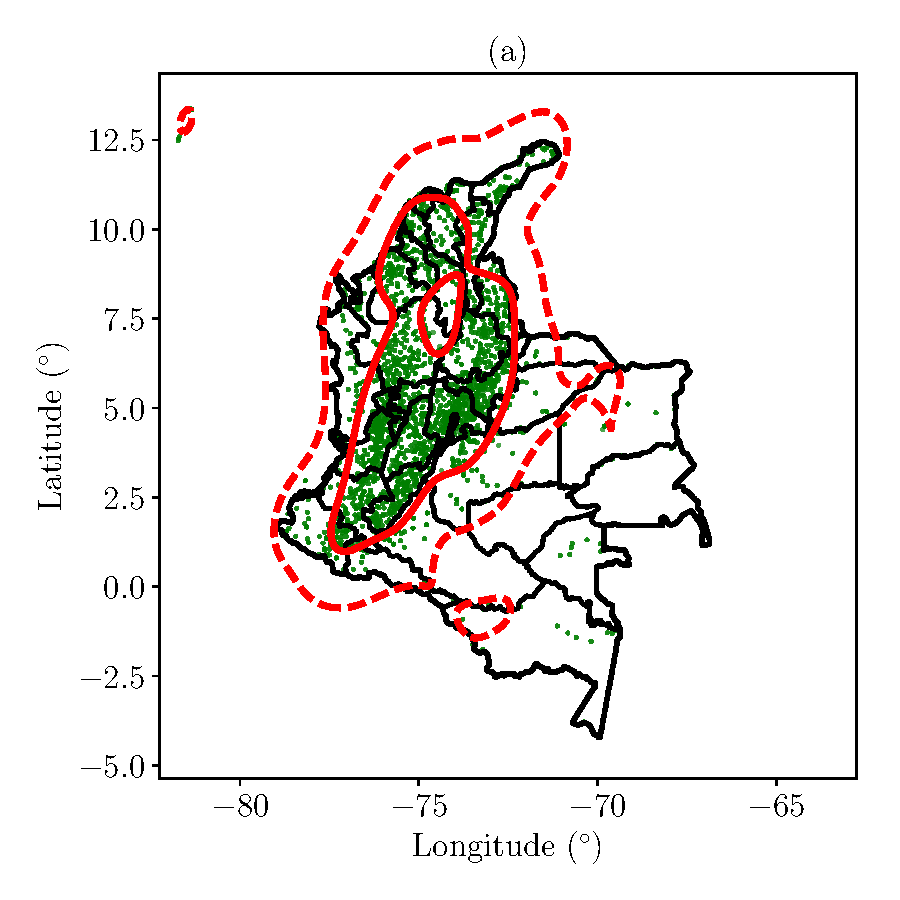
\includegraphics[scale=0.5]{totmap.pdf}
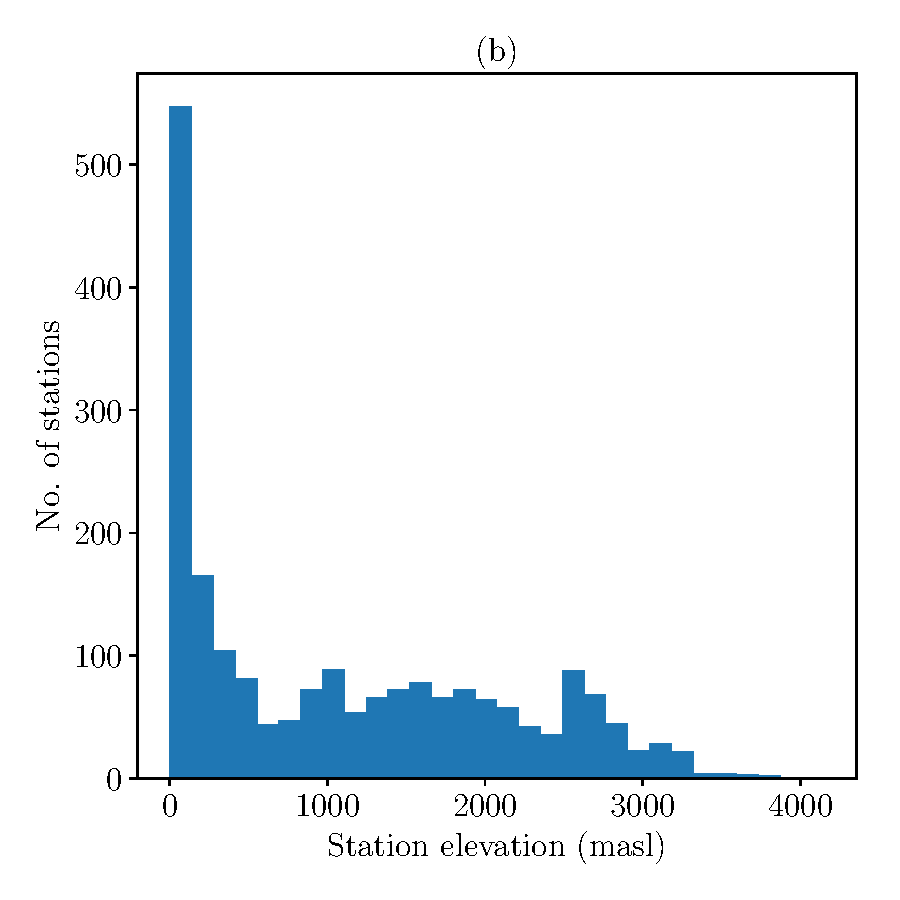
\includegraphics[scale=0.5]{elev.pdf}
\caption{Distribution of weather stations in the dataset. (a) 1$\sigma$ (solid) and 2$\sigma$ (dashed) countours of a gaussian kernel density estimation of the geographical distribution of weather stations (small green points) from the IDEAM 1980-2010 database. The estimation was done using the Python \texttt{scipy.stats.gaussian\_kde}  function. (b) Altitude histogram for all stations in the dataset.}\label{totmap}
\end{center}
\end{figure}



\begin{table}
\caption{\label{tabstype}Types of stations classified according to its measured variables.}
\begin{indented}
\item[]\begin{tabular}{@{}cccccc}
\br
Type&Precip.&Rain &Relative&Sunshine&No. of Stations\\
&&Days&Humidity&Duration&\\
\mr
$T_1$&Y&N&N&N&29\\
$T_2$&Y&Y&N&N&1563\\
$T_3$&Y&N&Y&N&1\\
$T_4$&Y&Y&Y&N&117\\
$T_5$&Y&N&N&Y&1\\
$T_6$&Y&Y&N&Y&8\\
$T_7$&Y&N&Y&Y&13\\
$T_8$&Y&Y&Y&Y&314\\
\br
\end{tabular}
\end{indented}
\end{table}

\section{Low-Dimensional Embedding of Climatological Data}

Our goal is to classify and group together stations that show a similar climatological behavior for each variable, regardless of the station's location, elevation or type. Since climate data track multi-annual seasonal variations, we can correlate weather patterns of regions which are not obviously related climatologically but might show a similar behavior, e.g. dry weather patterns in Guajira (a desert region in the north of Colombia) with similar dry conditions present at high-mountain sites in the Andes.\\

We classified stations using a low-dimensional embedding of the data \cite{embed} for each variable. This ensures that a classification algorithm can uncover features in the data even even when the data are projected across a number of dimensions that is lower than the native dimensionality of the data (which in this case is monthly, i.e. $N_\mathrm{dim}=12$). This involves applying a dimensionality reduction algorithm followed by a clustering algorithm. Given that we wish to make a grouping of stations showing similar climatological patterns without making too many assumptions on the data, we decided to use unsupervised learning techniques.  In our case, we chose Principal Component Analysis (PCA) covering 95\% of the variance followed by a Gaussian Mixture Model selected by a low/locally minimum Bayesian Information Criterion (BIC). 

\subsection{Principal Component Analysis}

We were able to reduce the dimensionality of the data for each variable from  $N_\mathrm{dim}=12$ to  $N_\mathrm{dim}^\mathrm{PCA}\le3$, while ensuring that at least 95\% of the variance of the data is explained by the least amount of components. For precipitation, rain days and sunshine duration, $N_\mathrm{dim}^\mathrm{PCA}(95\%)=3$ and for relative humidity $N_\mathrm{dim}^\mathrm{PCA}(95\%)=2$. To do this we used the Python \texttt{sklearn.decomposition.PCA} module \cite{sklearn}. Figure \ref{pcah} shows the relative humidity data projected across 2 principal components explaining 95\% of the variance, thus preserving most of the original structure of the data.

\begin{figure}
\begin{center}
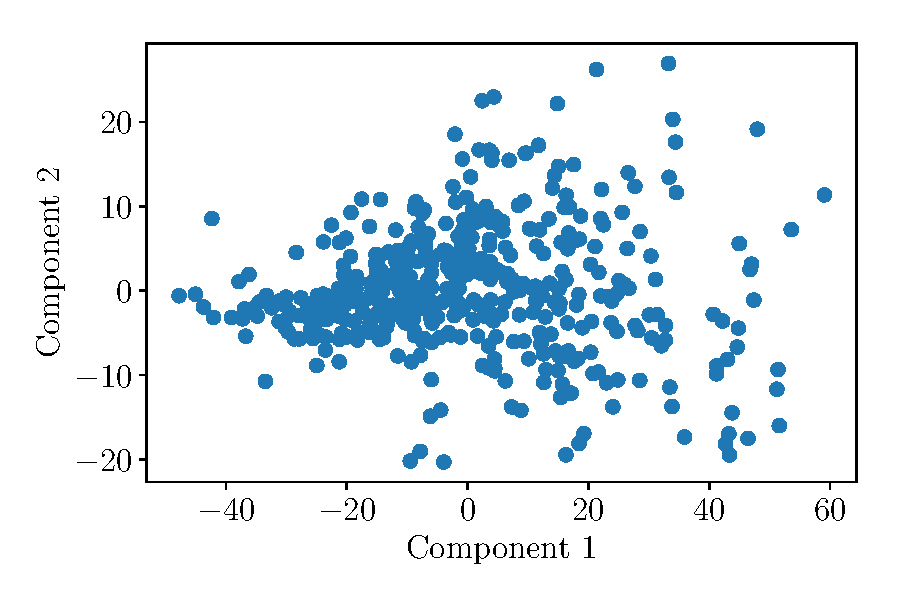
\includegraphics[scale=0.8]{pcah.pdf}
\caption{Relative humidity data projected across 2 principal components. The dimensionality of the data has been reduced from 12 to 2 while covering 95\% of the variance of the data. }\label{pcah}
\end{center}
\end{figure}

\subsection{Gaussian Mixture Models}

After projecting the data along the components found by the PCA algorithm, we clustered the dimensionally-reduced data using a Gaussian Mixture Model, which uses an Expectation-Maximization algorithm to find a Maximum Likelihood model composed of a number $N_\mathrm{G-C}$ of Gaussian distributions, each of which represents a cluster in the data \cite{gmm}. Depending on the restrictions put on the covariance of each Gaussian distribution across the data space, the number of free parameters can go from $N_\mathrm{G-C}(N_\mathrm{dim}+1)$ (spherical covariance) to  $N_\mathrm{G-C}(3N_\mathrm{dim}+1)$ (full covariance). Since the number of components and covariance restriction is given by the user and not \emph{a posteriori} by the algorithm, me need to make sure that the Gaussian components do not over-fit the data, e.g. a model which yields one cluster per datum should be disallowed.\\

In order to achieve this, we compare the Bayesian Information Criterion \cite{bicref} for a grid of Gaussian clusters ($N_\mathrm{G-C}<20$) and covariance restriction methods for each variable (Figure \ref{bic}). To do this we used the Python \texttt{sklearn.mixture.GMM} module \cite{sklearn}. We selected the models which produced the lowest BIC value, and plotted the GMM-classified, PCA-projected climate data in Figure \ref{lde}. \\

From the climatological clusters in Figures \ref{clusth}-\ref{clustb} we selected clusters that indicate a dry, sunny climate. Table \ref{tabclu} shows the selected number of clusters and covariance method for each variable along with our preferred clusters . From here on, if a station appears in one of our preferred clusters, we will say that it satisfies our criterion for that specific variable.\\

\begin{figure}
\begin{center}
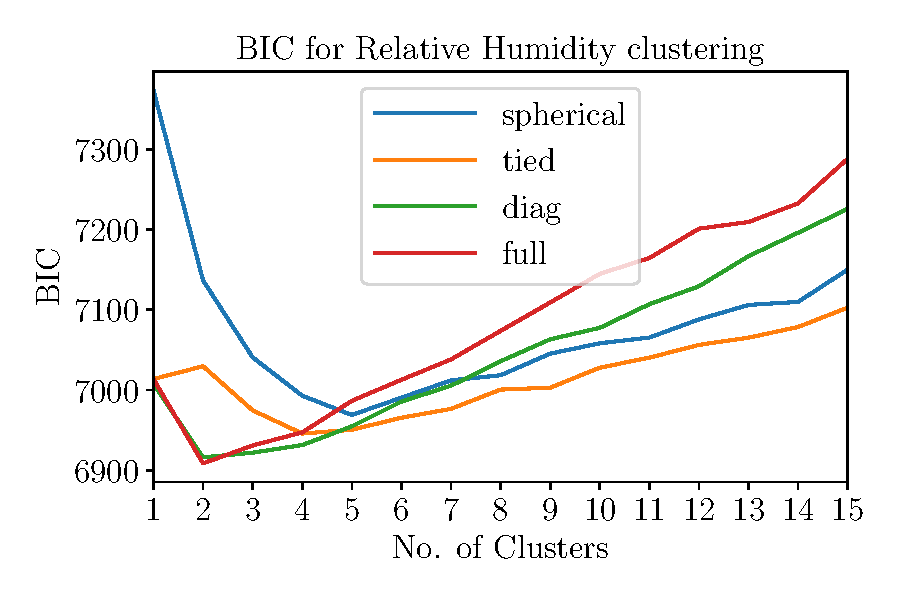
\includegraphics[scale=0.5]{bich.pdf}
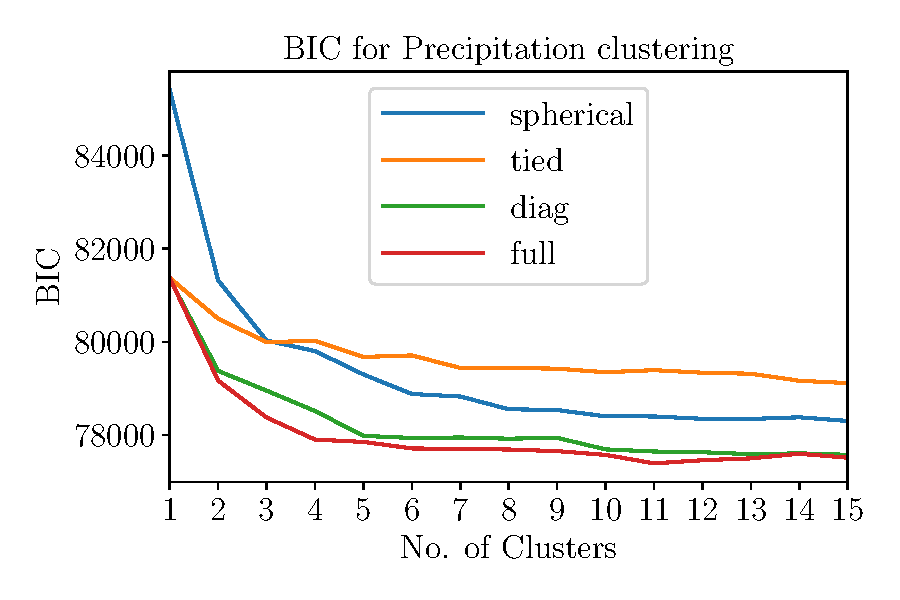
\includegraphics[scale=0.5]{bicl.pdf}\\
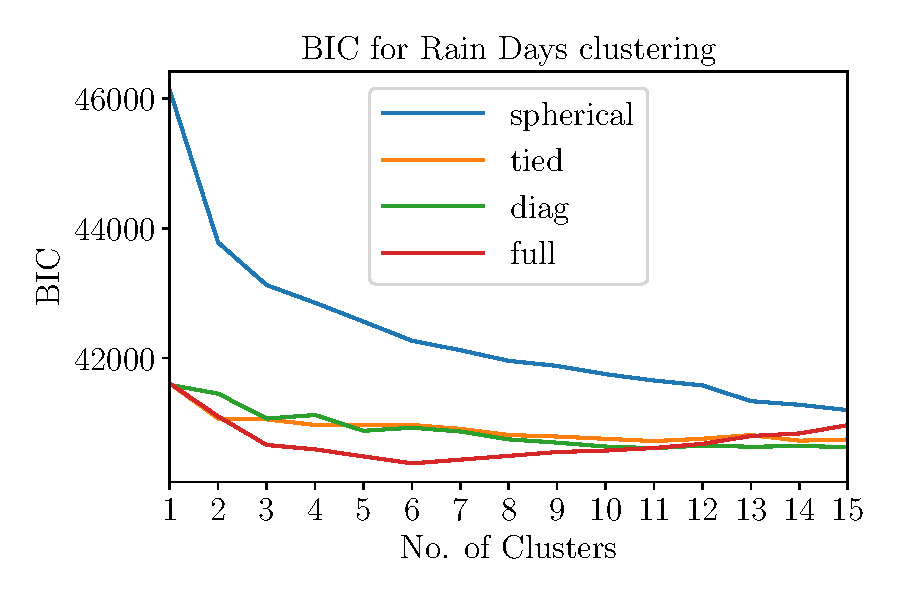
\includegraphics[scale=0.5]{bicd.pdf}
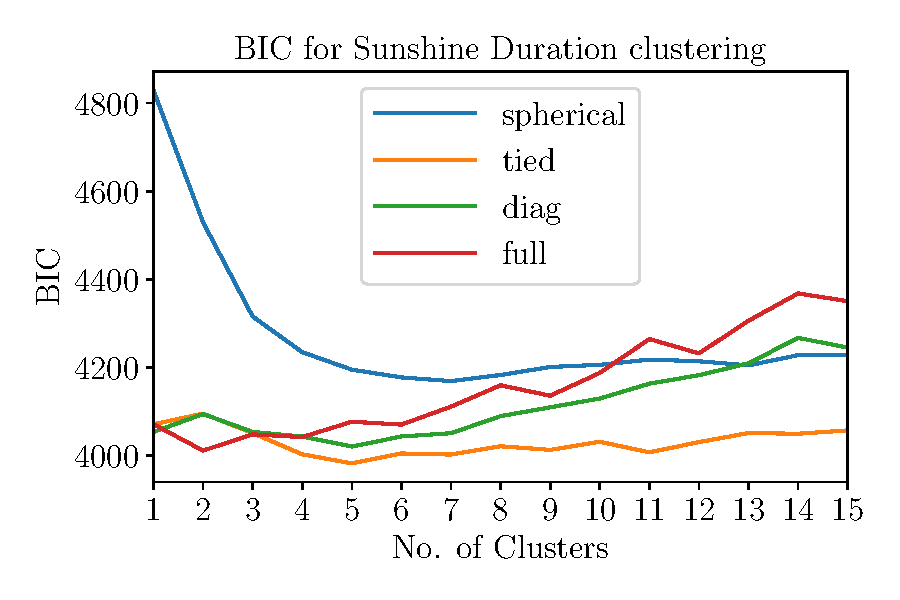
\includegraphics[scale=0.5]{bicb.pdf}
\caption{Bayesian Information Criterion (BIC) results for Gaussian Mixture Models using a different number of clusters and using different covariance restriction methods applied on each measured variable dataset.}\label{bic}
\end{center}
\end{figure}





\begin{figure}
\begin{center}
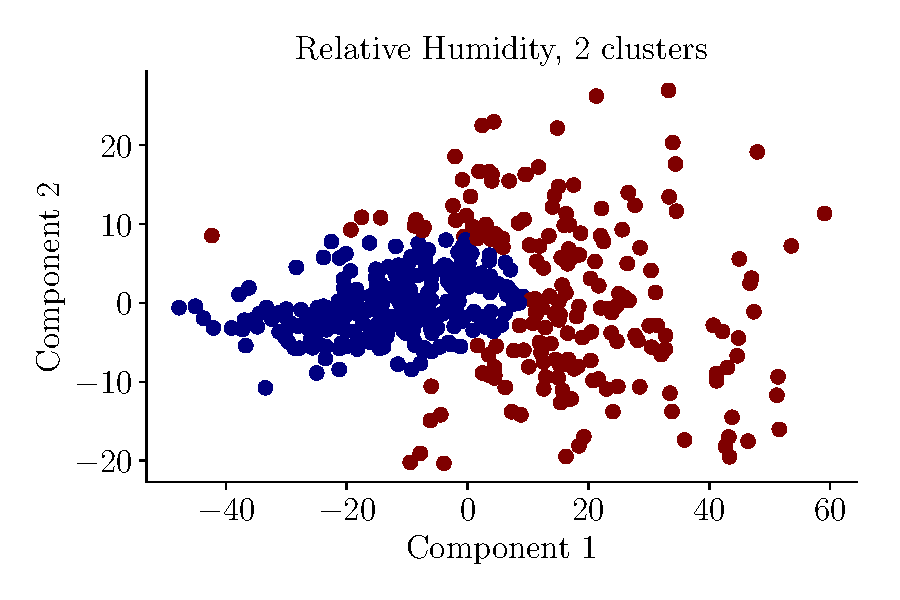
\includegraphics[scale=0.5]{ldeh.pdf}
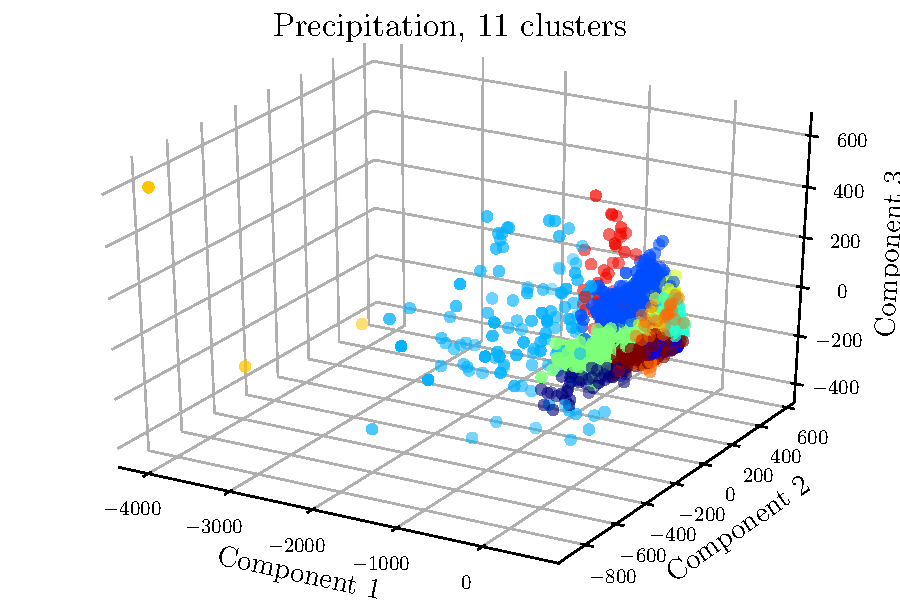
\includegraphics[scale=0.5]{ldel.pdf}
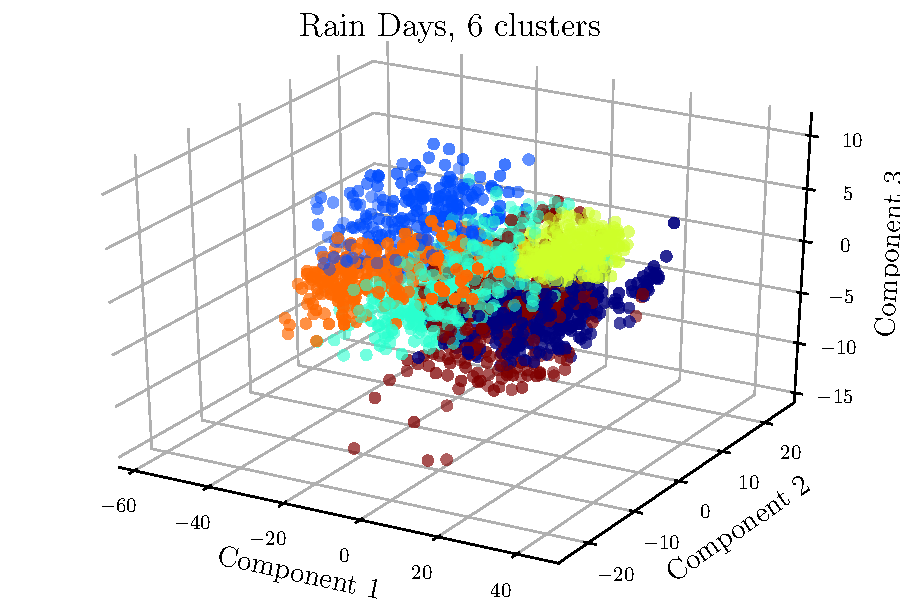
\includegraphics[scale=0.5]{lded.pdf}
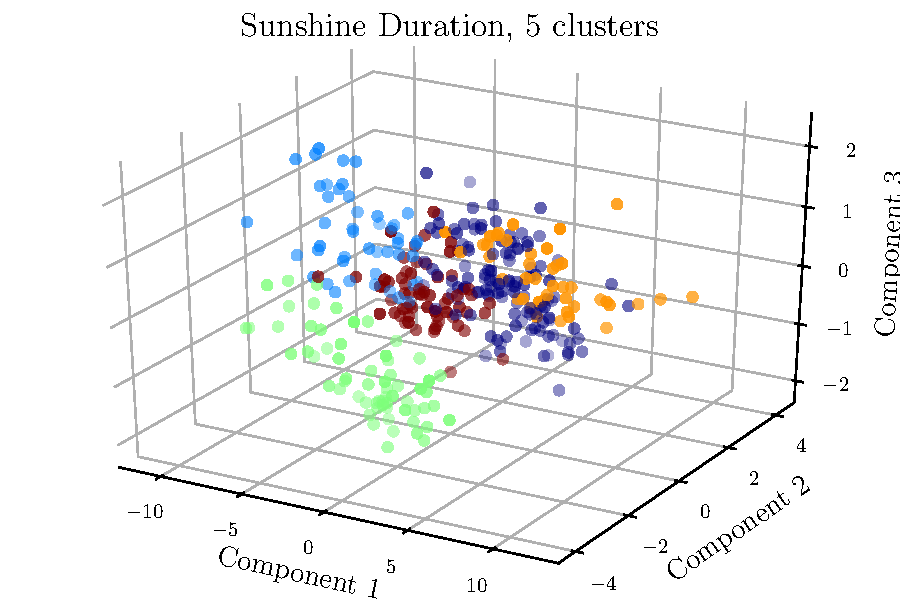
\includegraphics[scale=0.5]{ldeb.pdf}
\caption{Lowest BIC Gaussian Mixture Model clustering of reduced dimensionality climate data. Colors indicate the results of the clustering classification.}\label{lde}
\end{center}
\end{figure}

\begin{figure}
\begin{center}
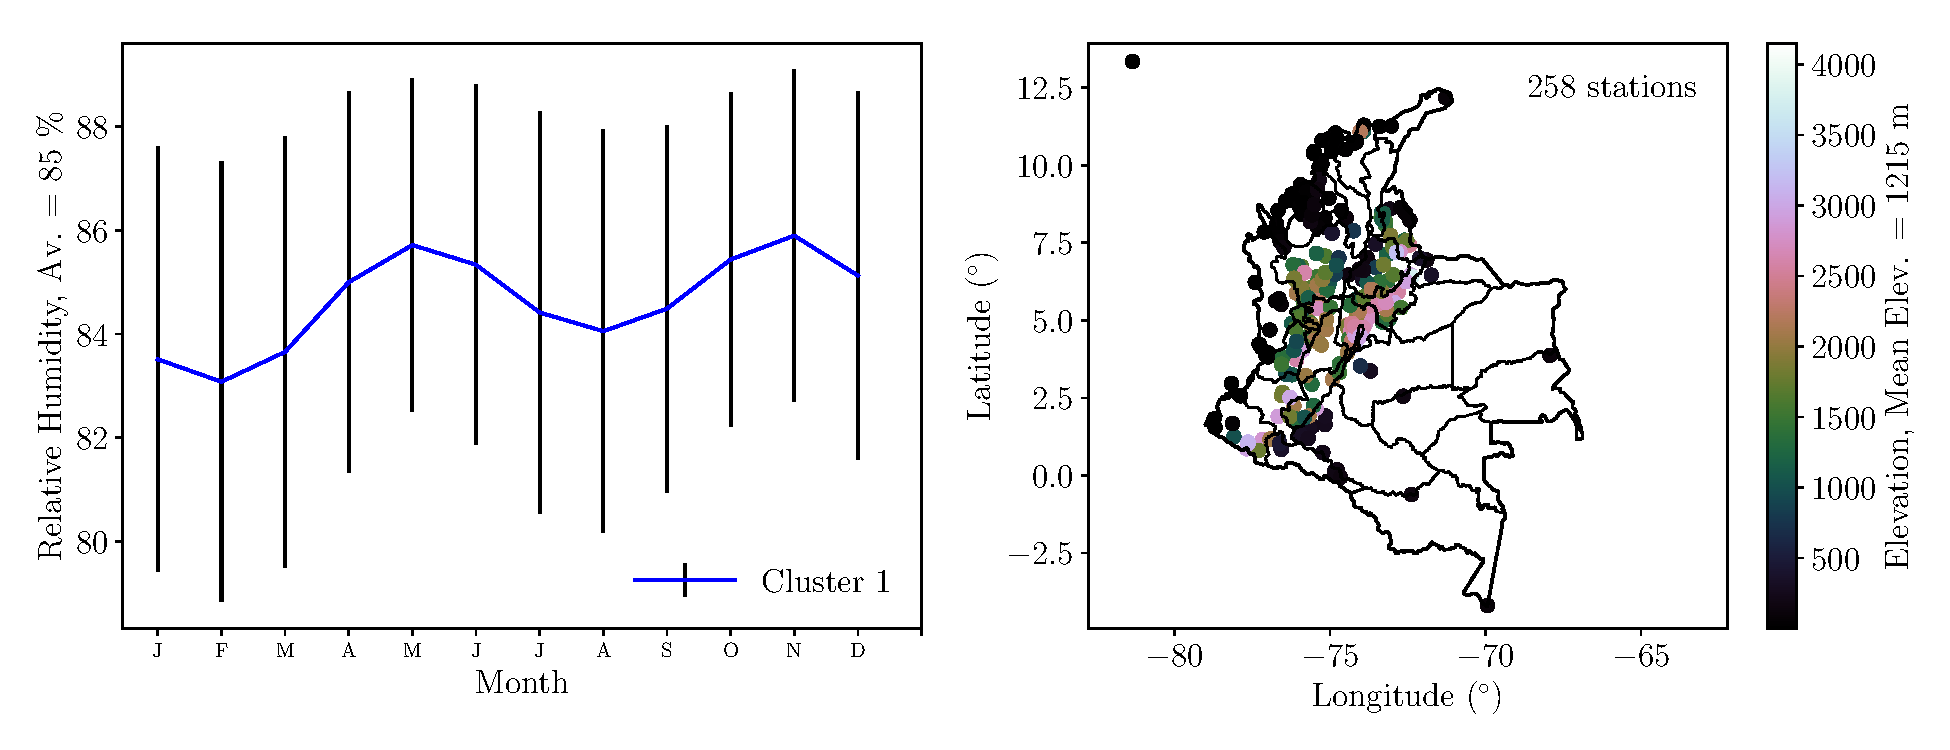
\includegraphics[scale=0.5]{gmmh0.pdf}
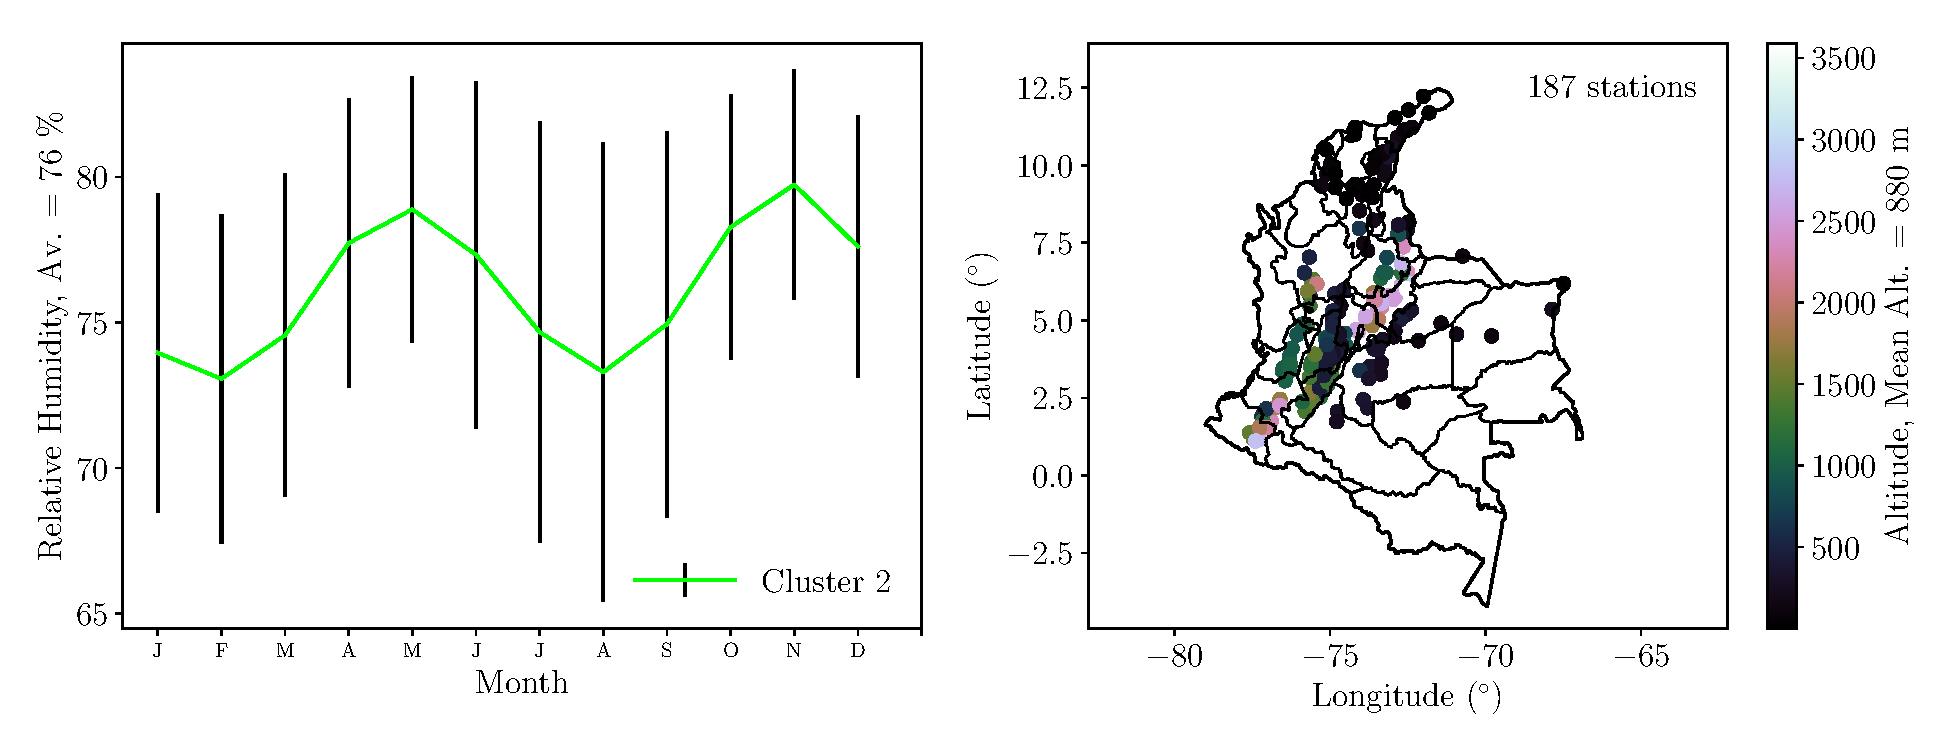
\includegraphics[scale=0.5]{gmmh1.pdf}
\caption{Climate clusters as predicted by the lowest-BIC Gaussian Mixture Model for relative humidity. Left column: Average monthly relative humidity and standard deviation (error bars) for each climate cluster. Right column: Geographical location and altitude of weather stations in each relative humidity cluster.}\label{clusth}
\end{center}
\end{figure}

\begin{figure}
\begin{center}
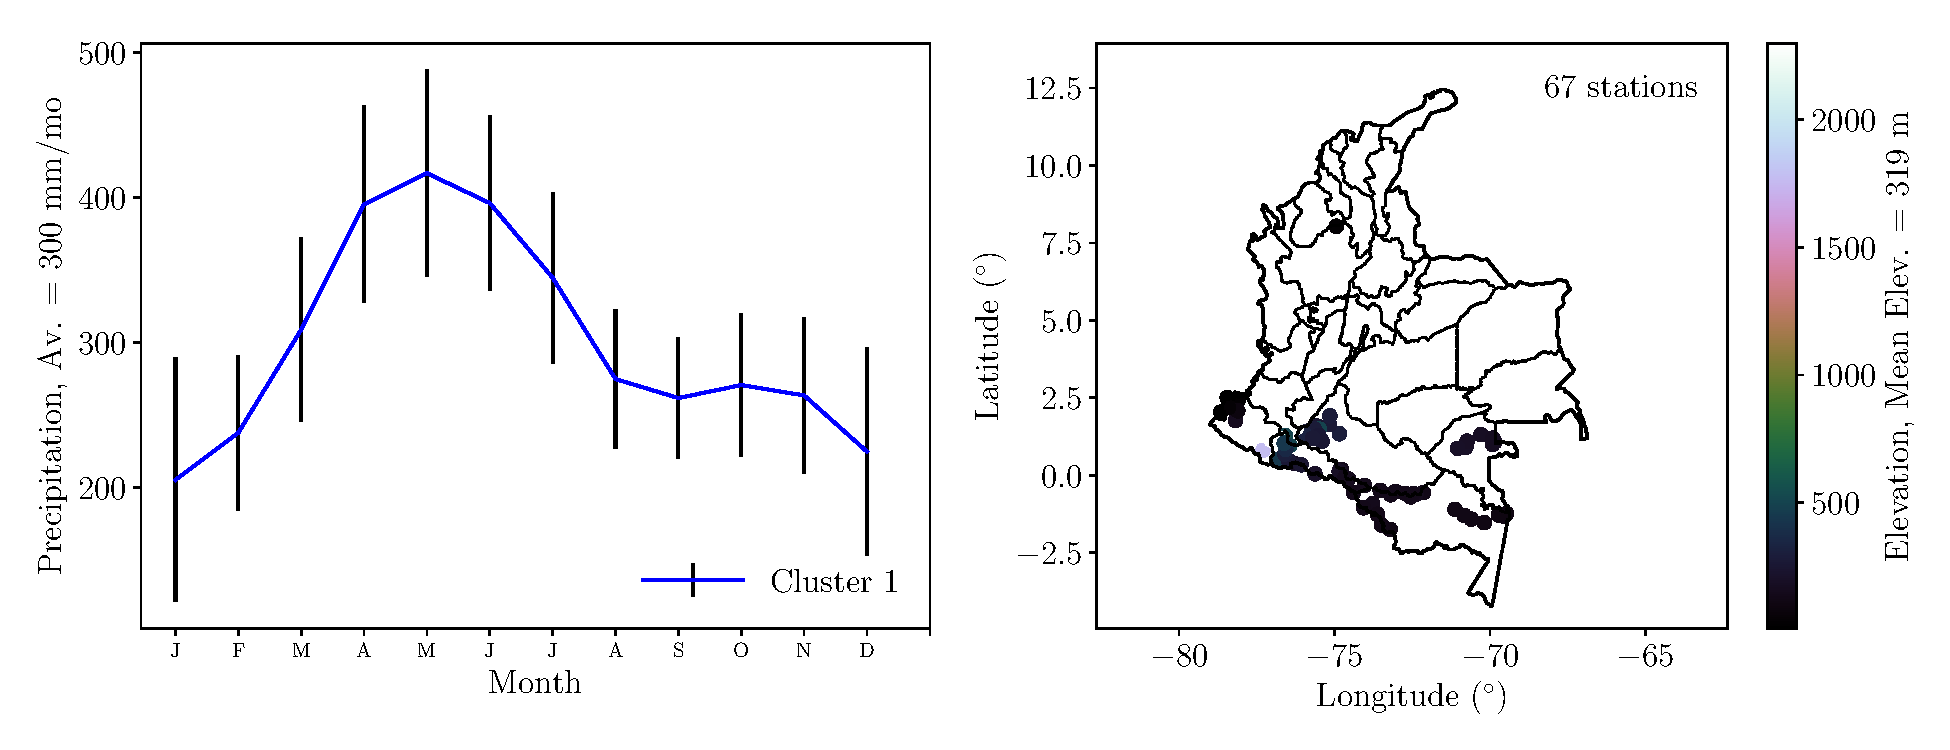
\includegraphics[scale=0.5]{gmml0.pdf}
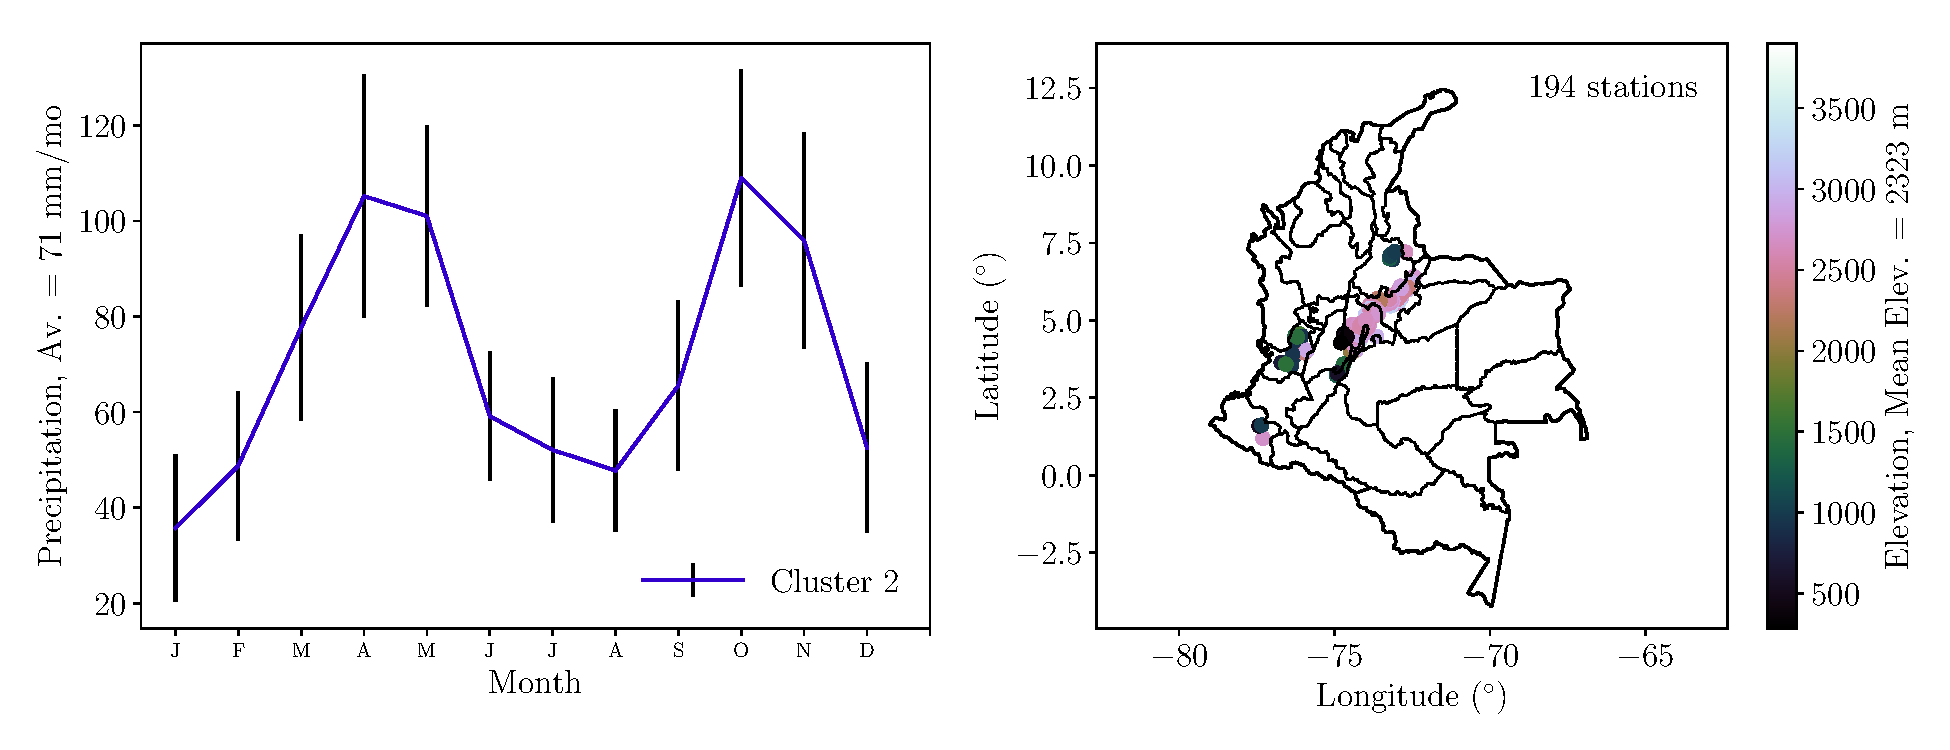
\includegraphics[scale=0.5]{gmml1.pdf}
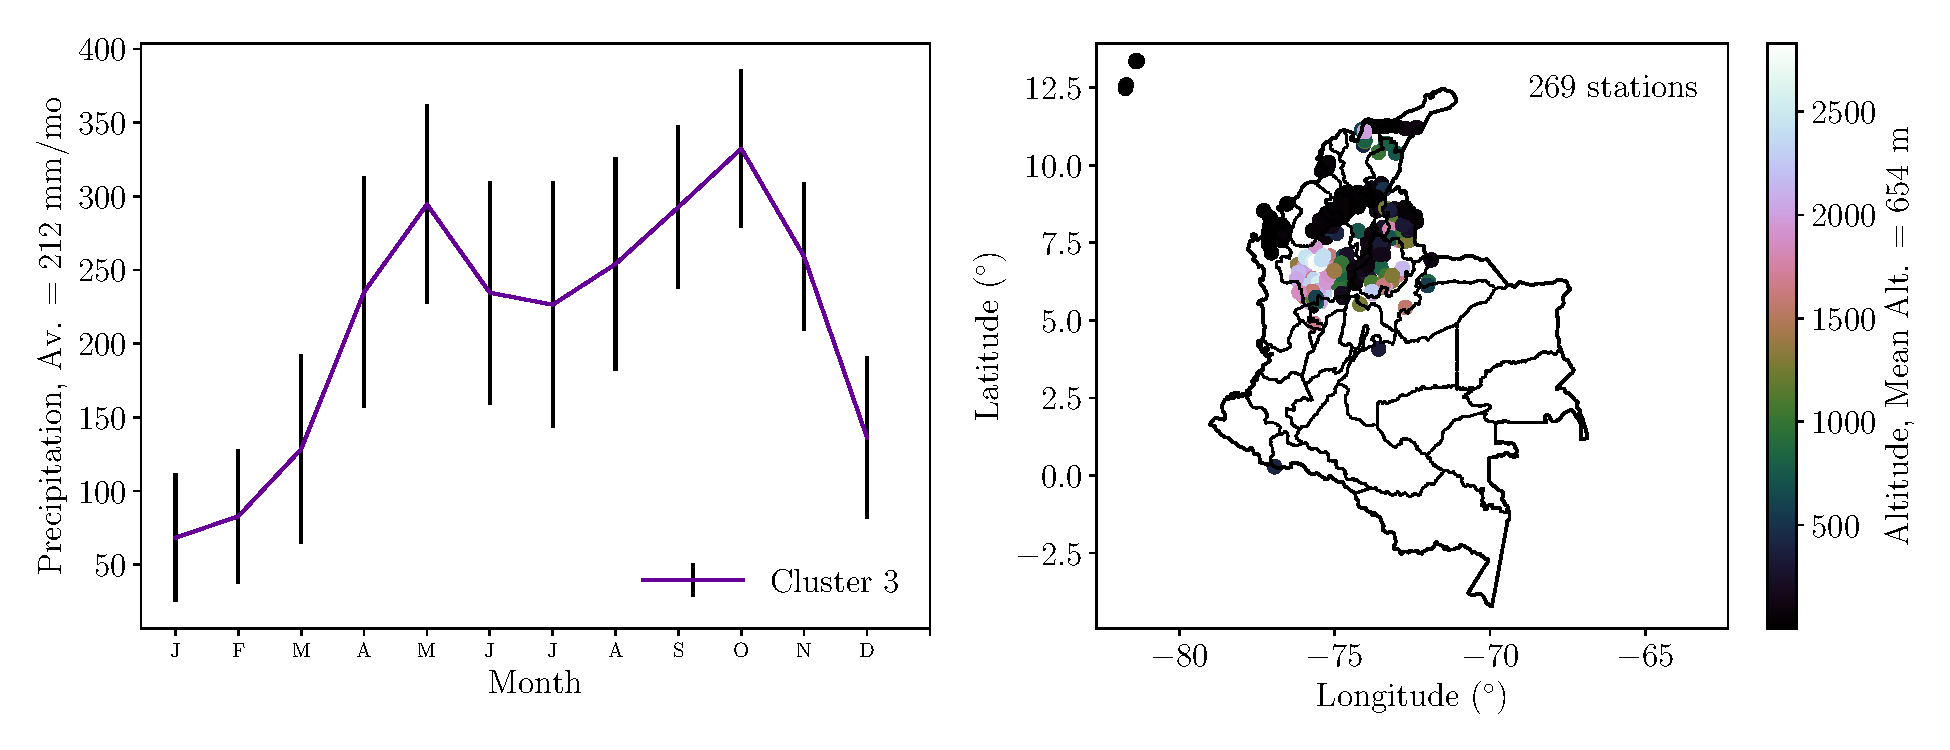
\includegraphics[scale=0.5]{gmml2.pdf}
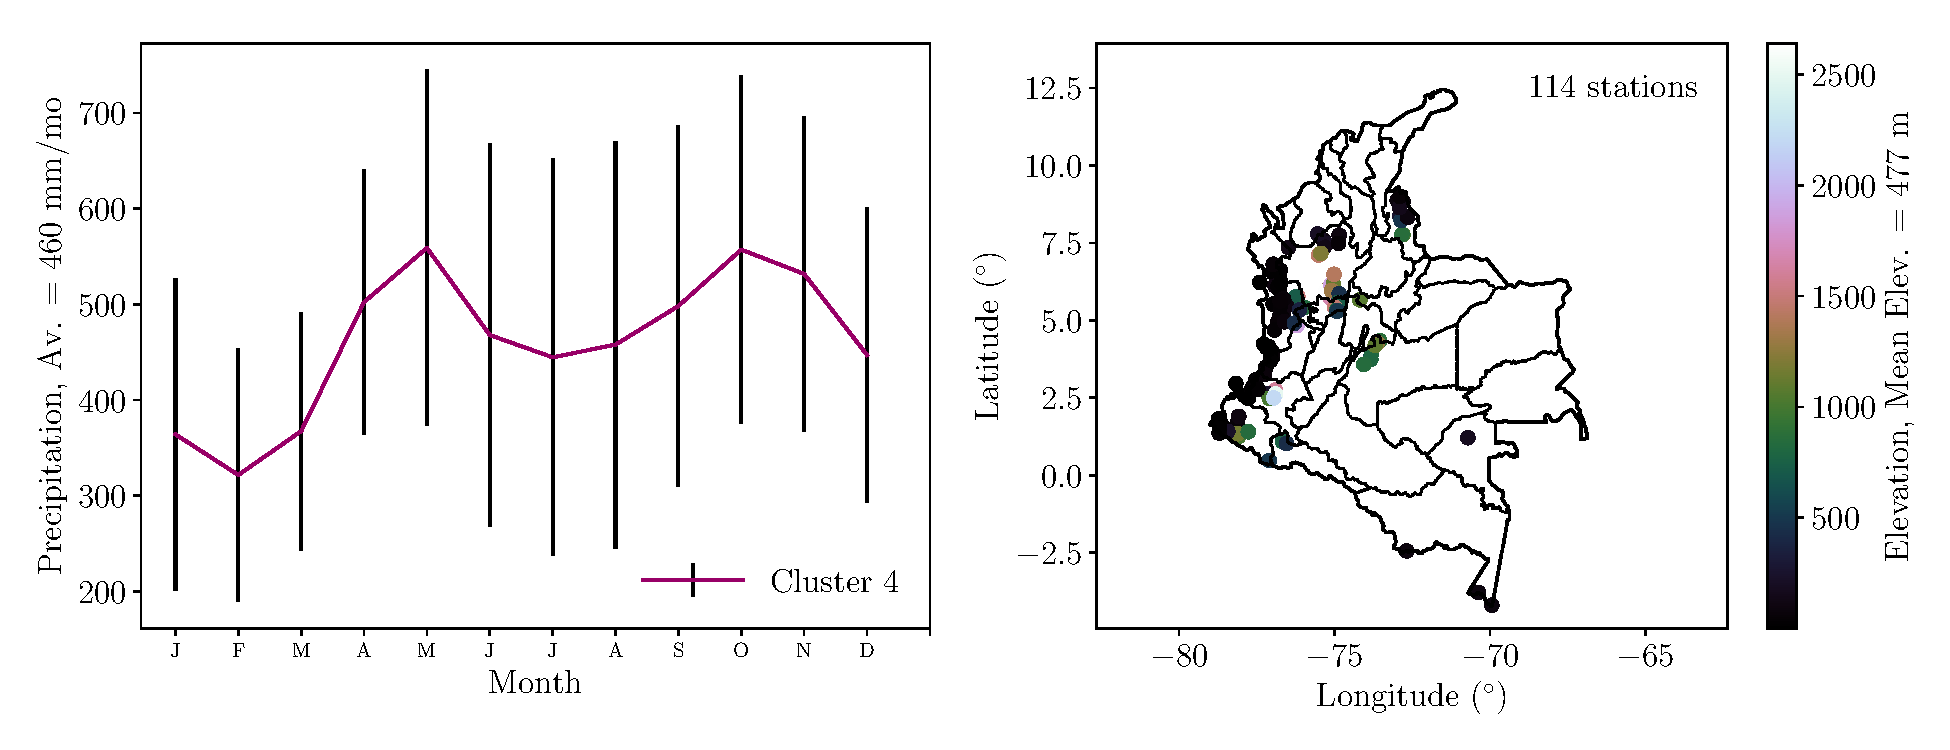
\includegraphics[scale=0.5]{gmml3.pdf}
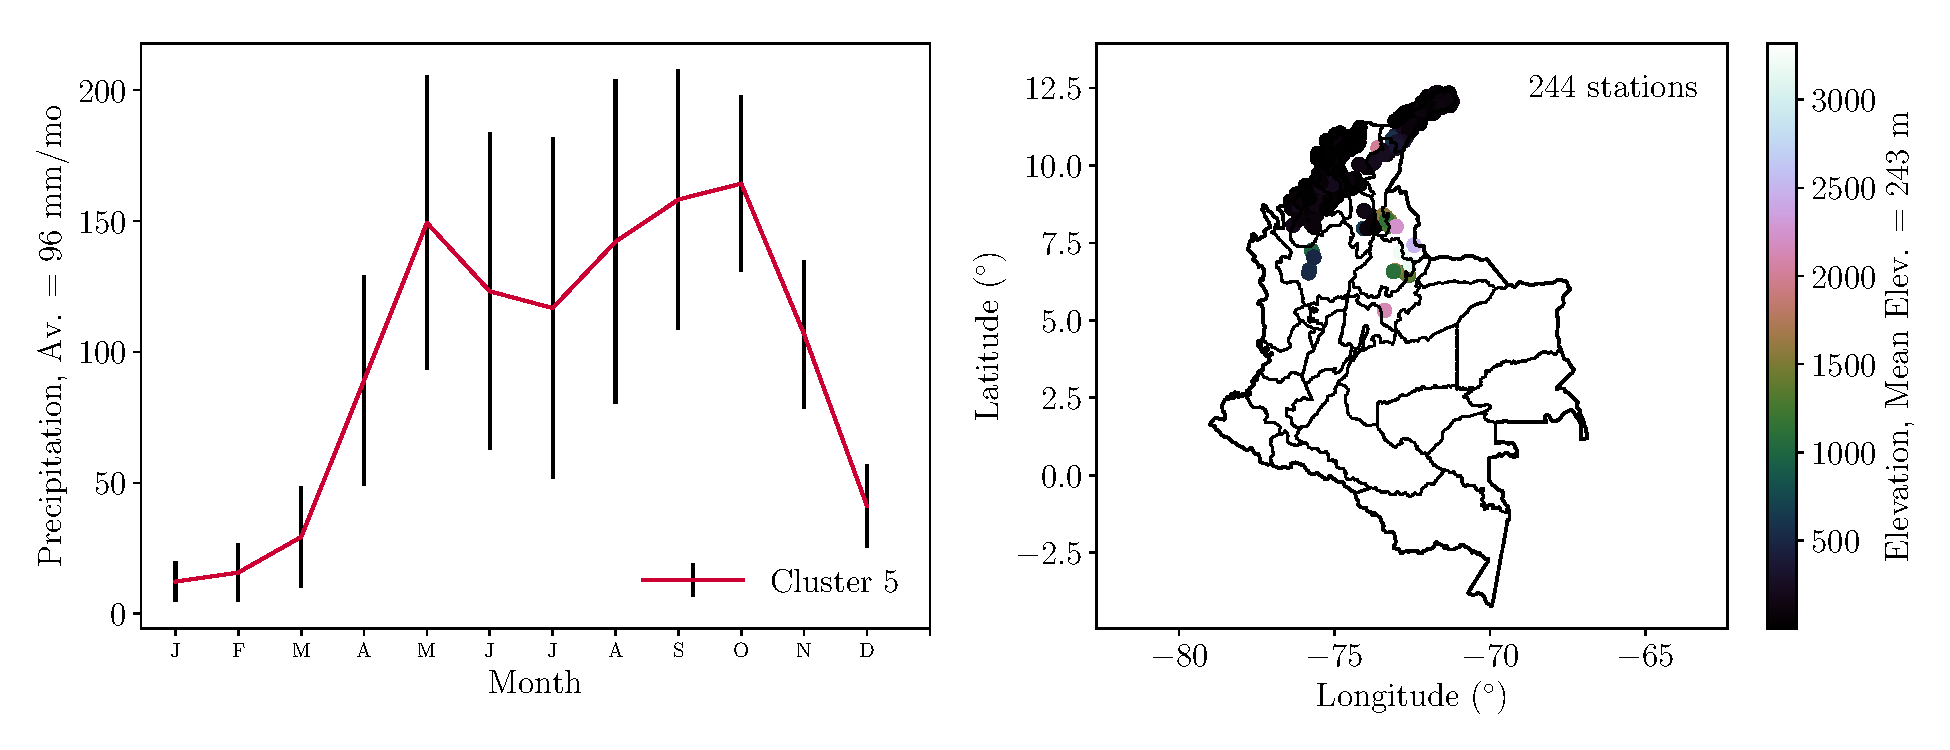
\includegraphics[scale=0.5]{gmml4.pdf}
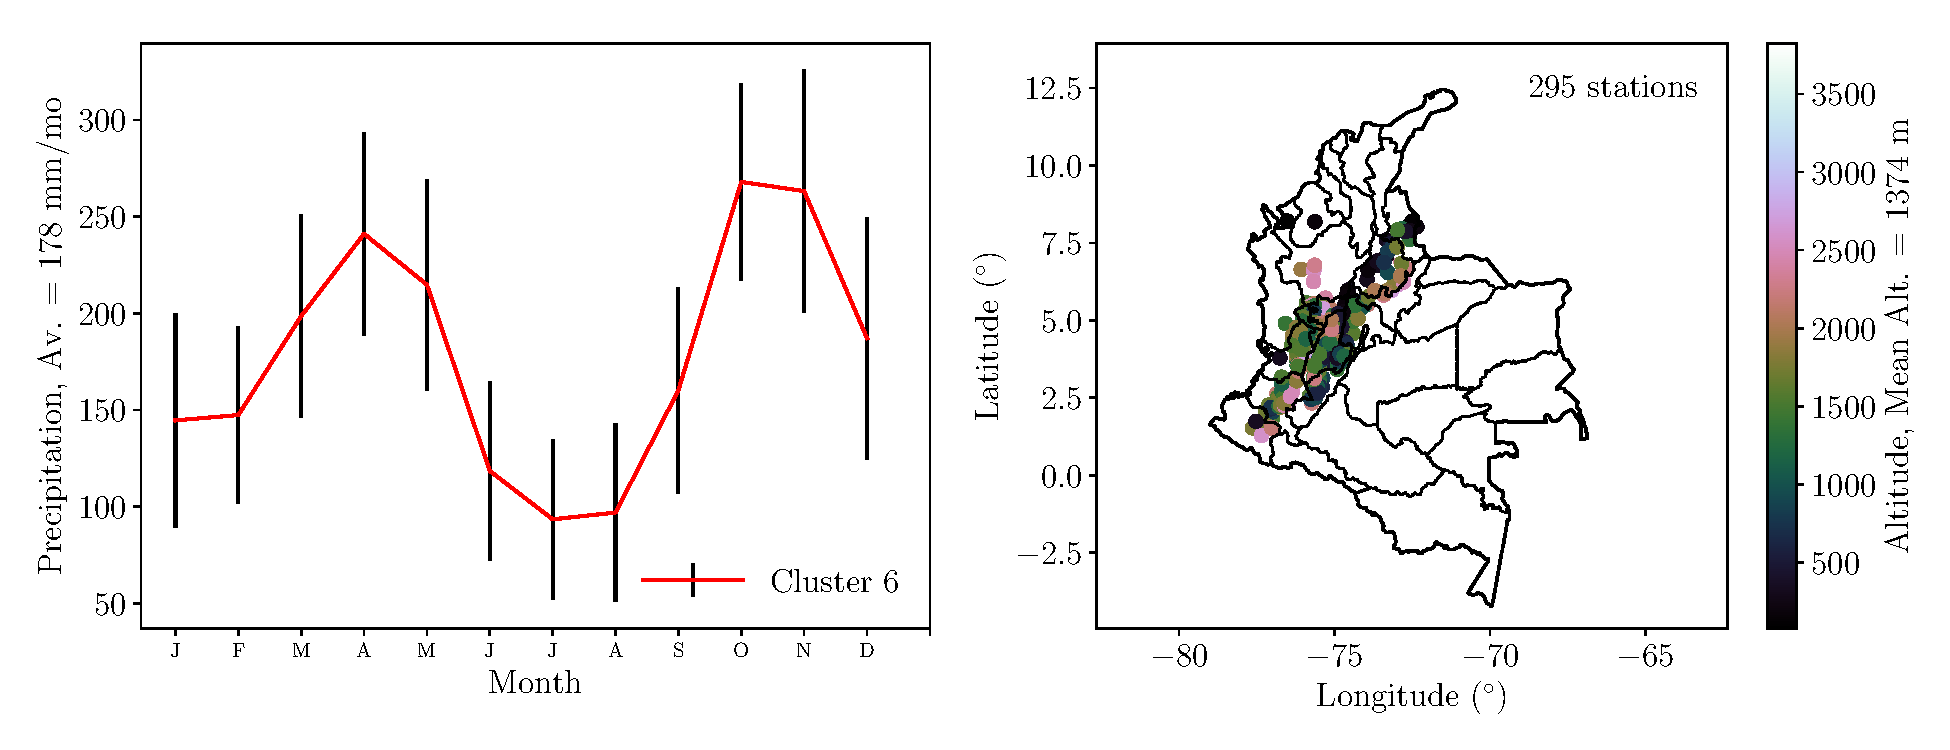
\includegraphics[scale=0.5]{gmml5.pdf}
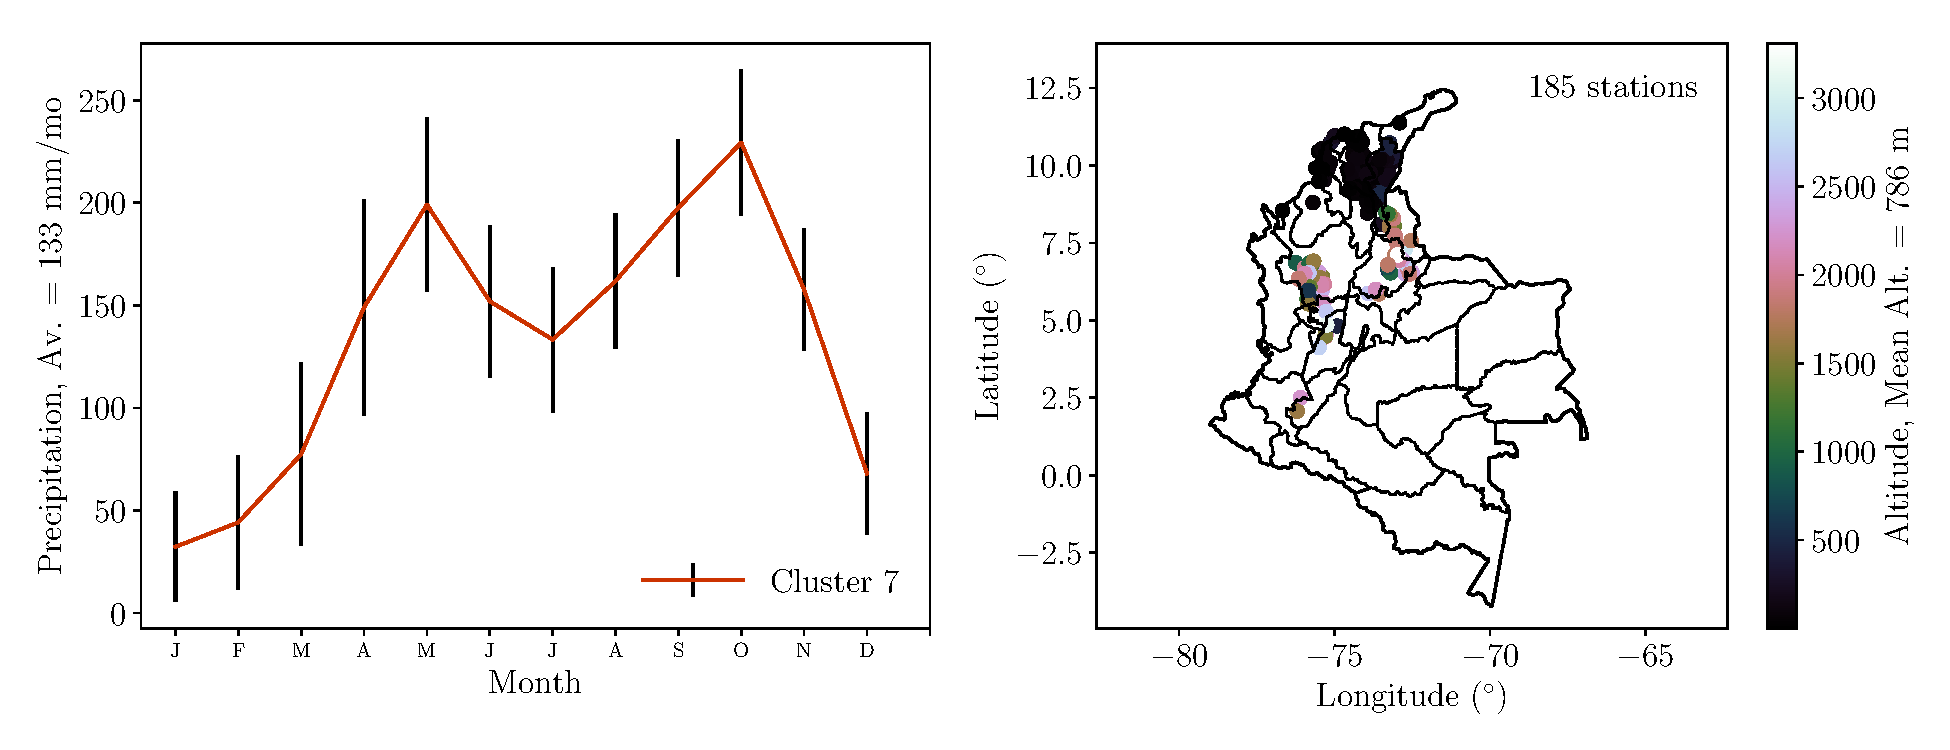
\includegraphics[scale=0.5]{gmml6.pdf}
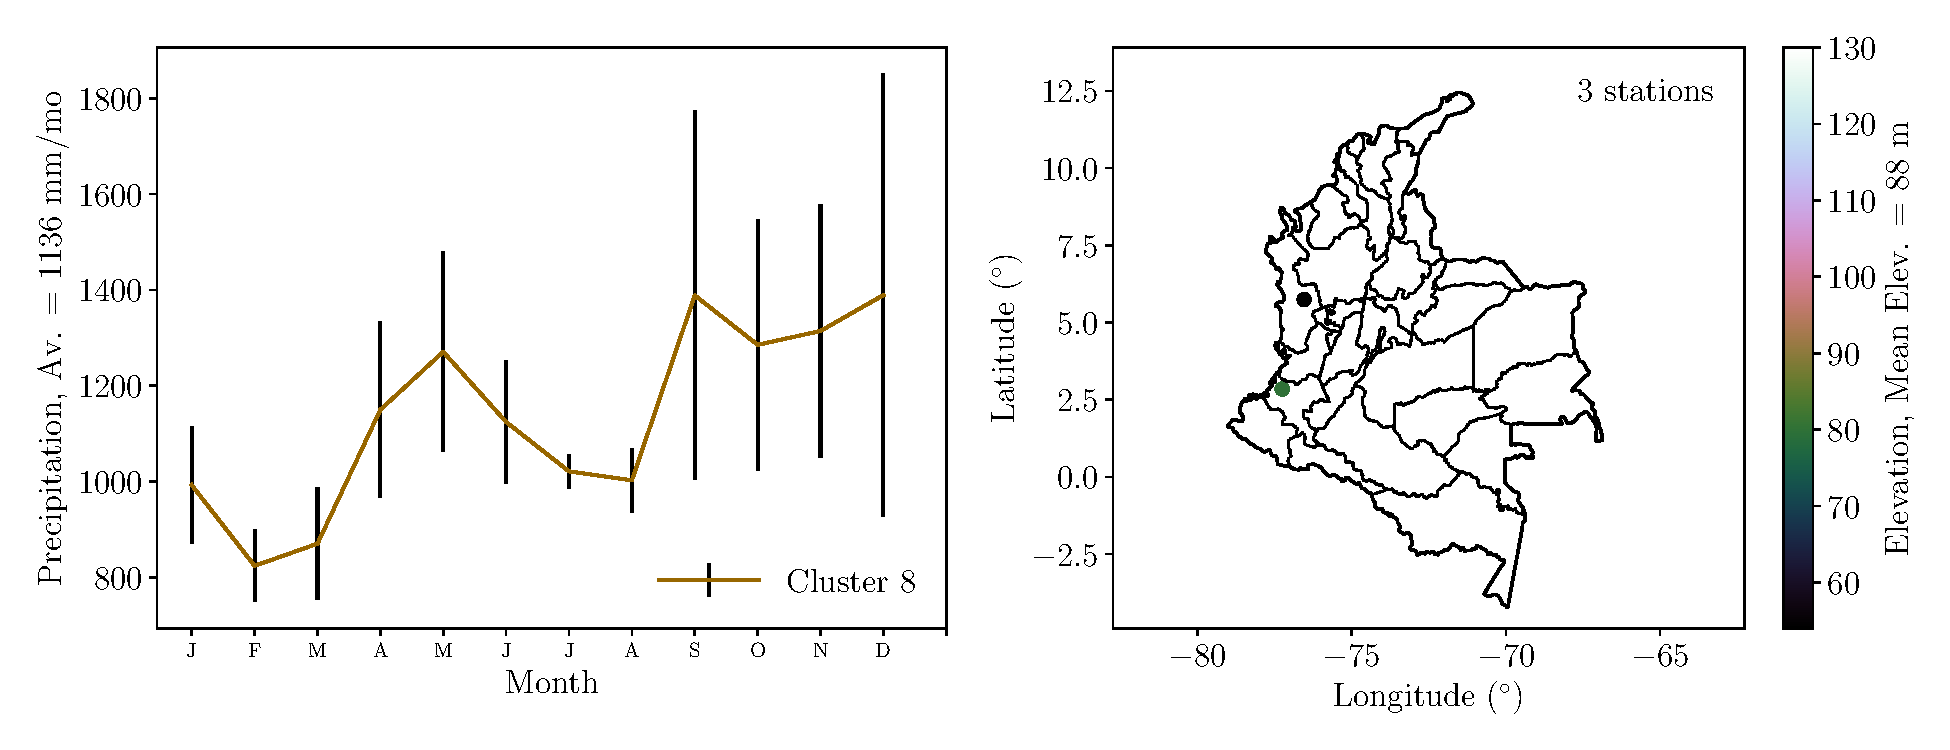
\includegraphics[scale=0.5]{gmml7.pdf}
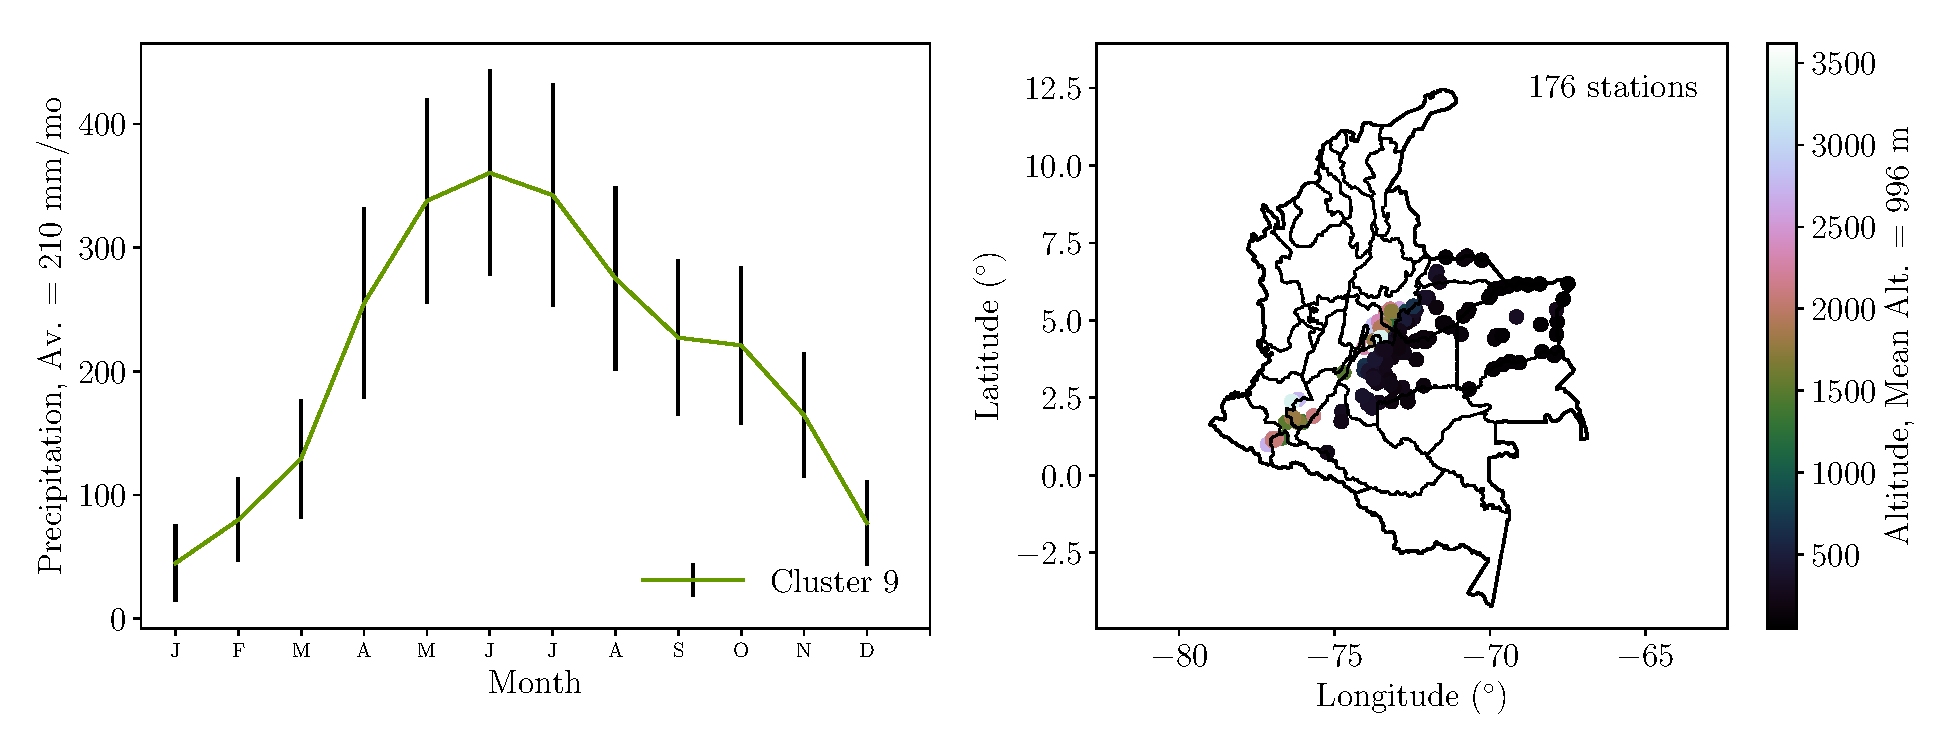
\includegraphics[scale=0.5]{gmml8.pdf}
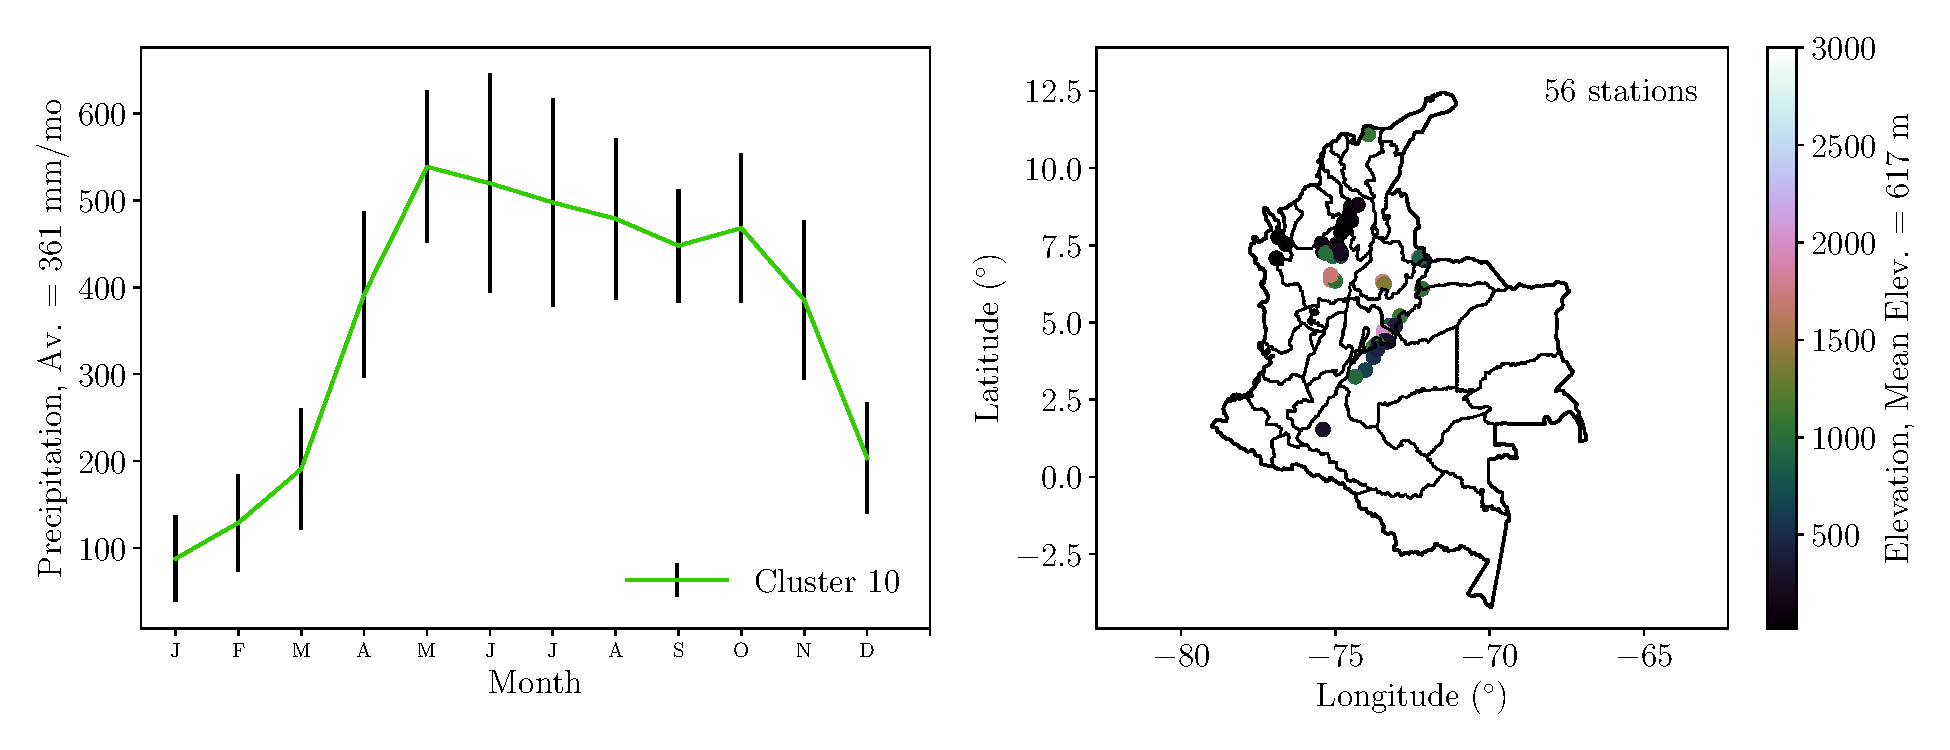
\includegraphics[scale=0.5]{gmml9.pdf}
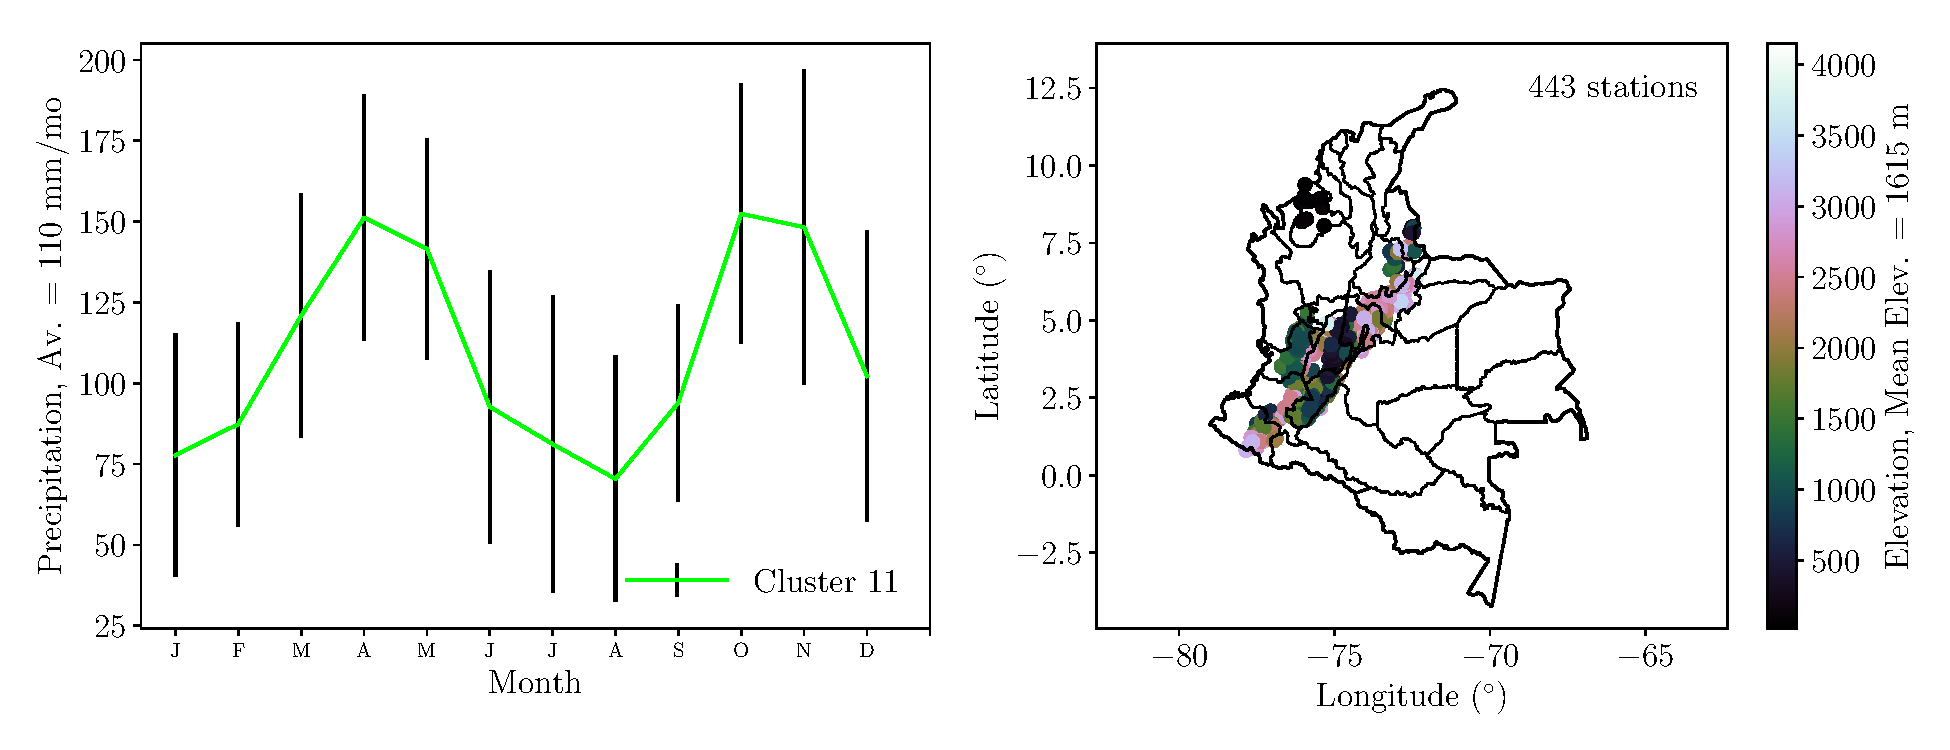
\includegraphics[scale=0.5]{gmml10.pdf}
\caption{Climate clusters as predicted by the lowest-BIC Gaussian Mixture Model for precipitation. Left column: Average monthly precipitation and standard deviation (error bars) for each climate cluster. Right column: Geographical location and altitude of weather stations in each precipitation cluster.}\label{clustl}
\end{center}
\end{figure}

\begin{figure}
\begin{center}
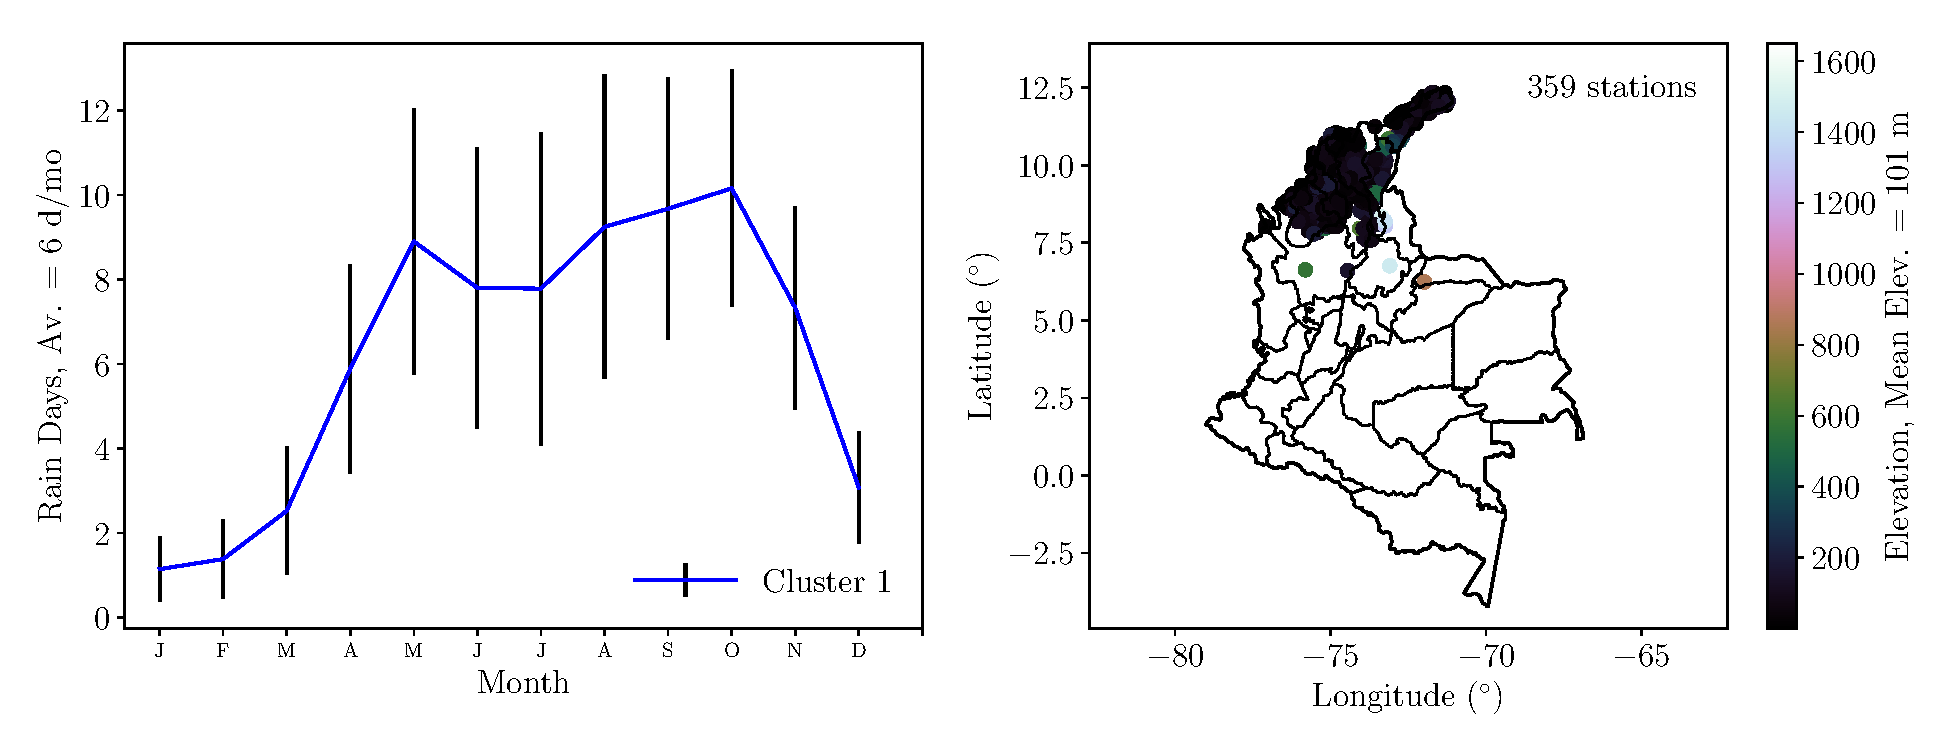
\includegraphics[scale=0.5]{gmmd0.pdf}
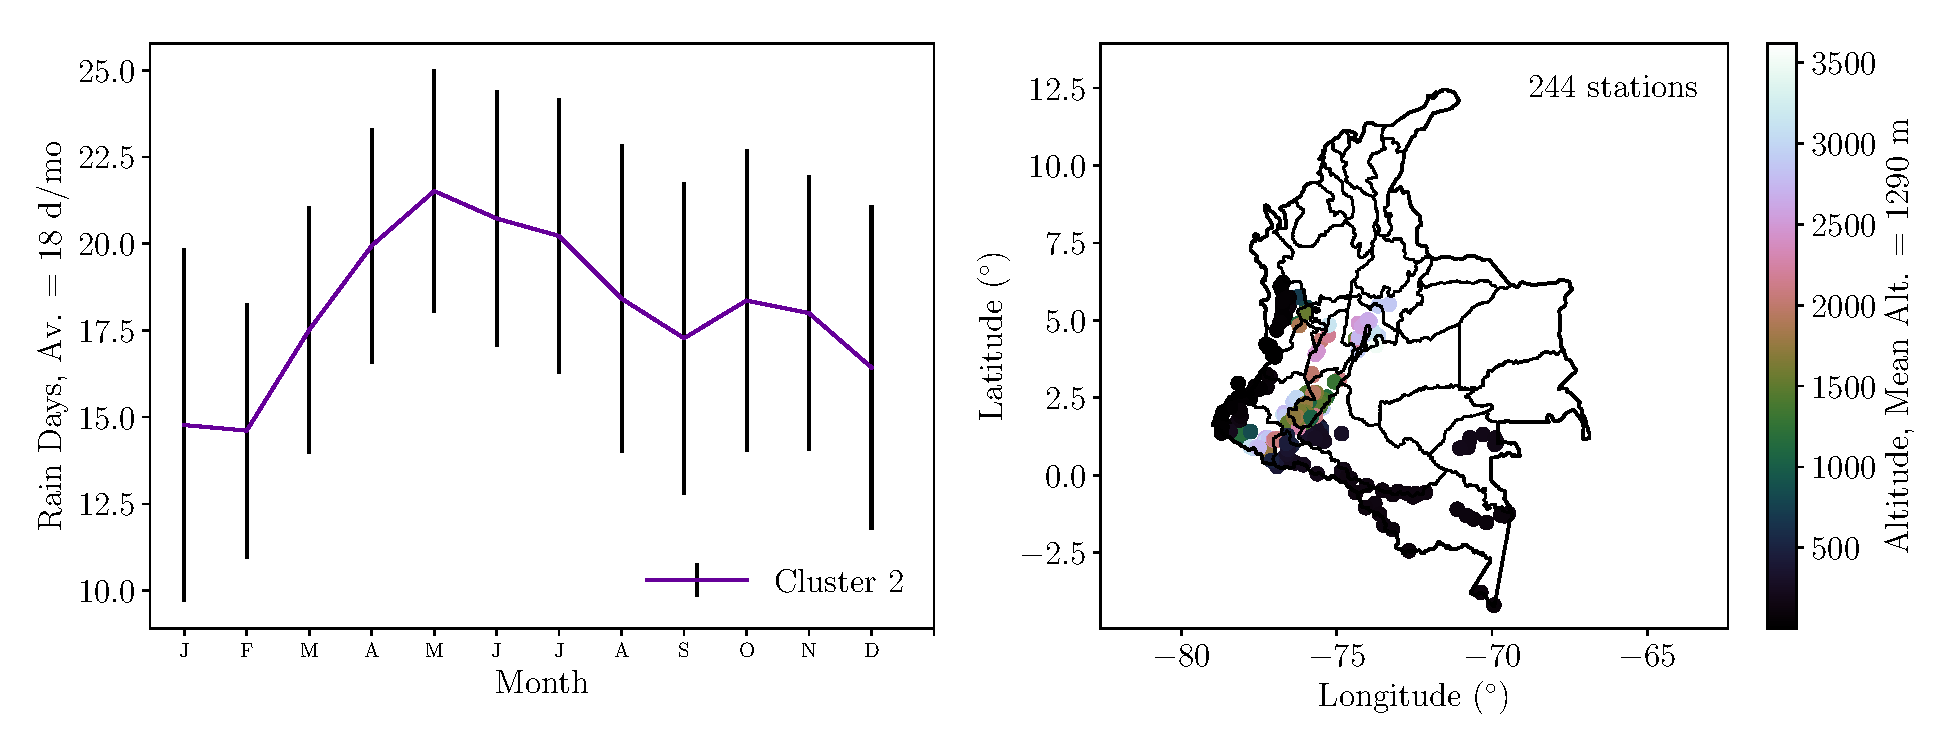
\includegraphics[scale=0.5]{gmmd1.pdf}
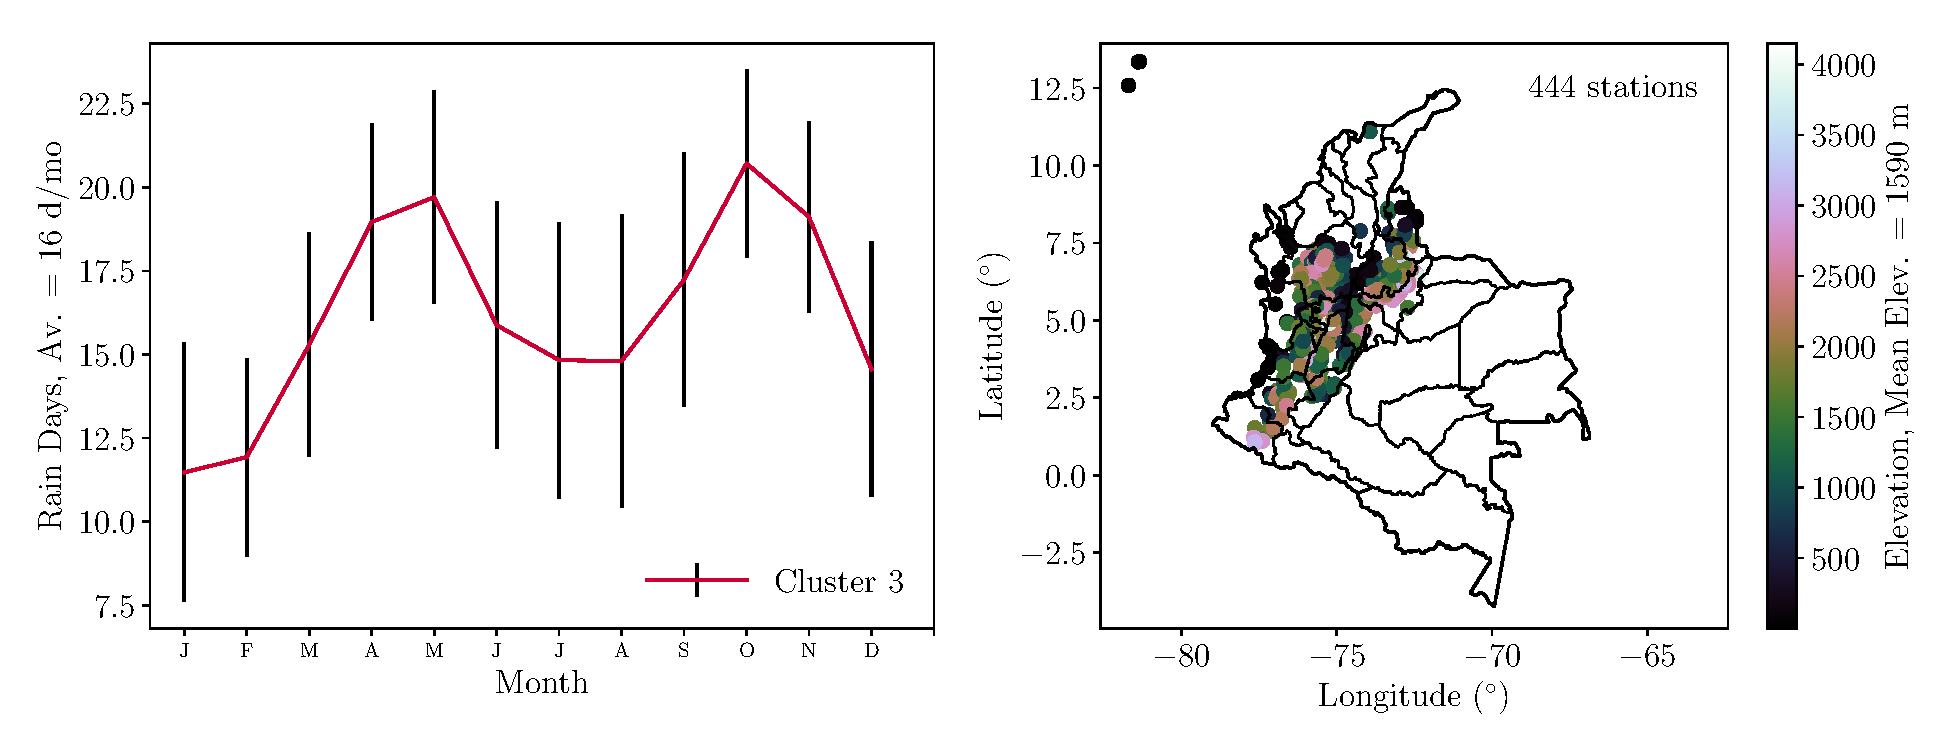
\includegraphics[scale=0.5]{gmmd2.pdf}
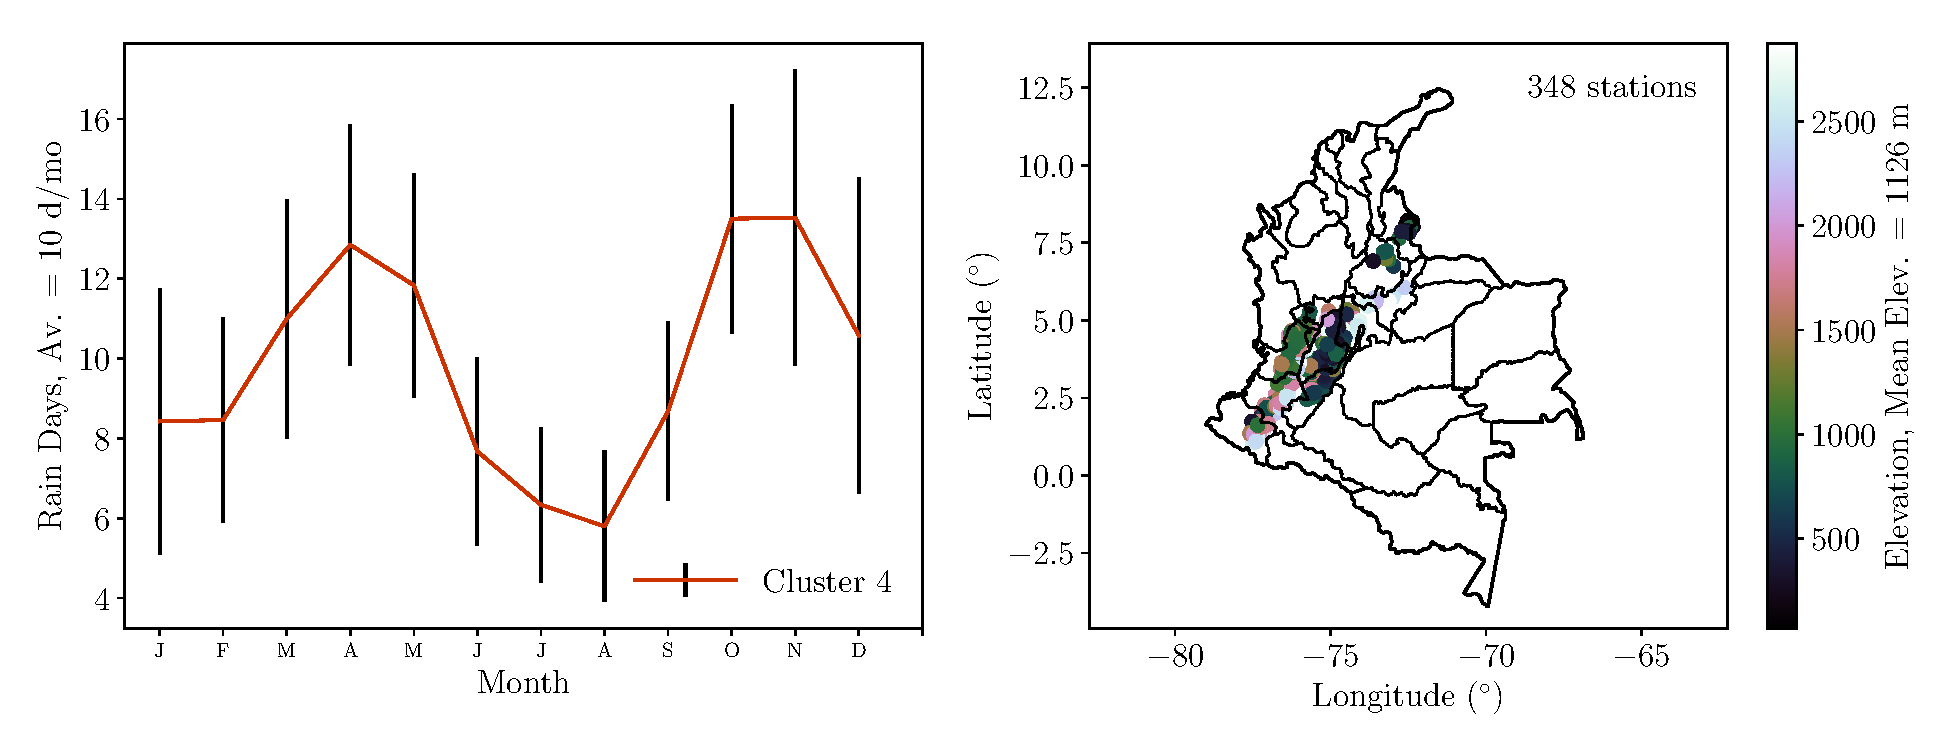
\includegraphics[scale=0.5]{gmmd3.pdf}
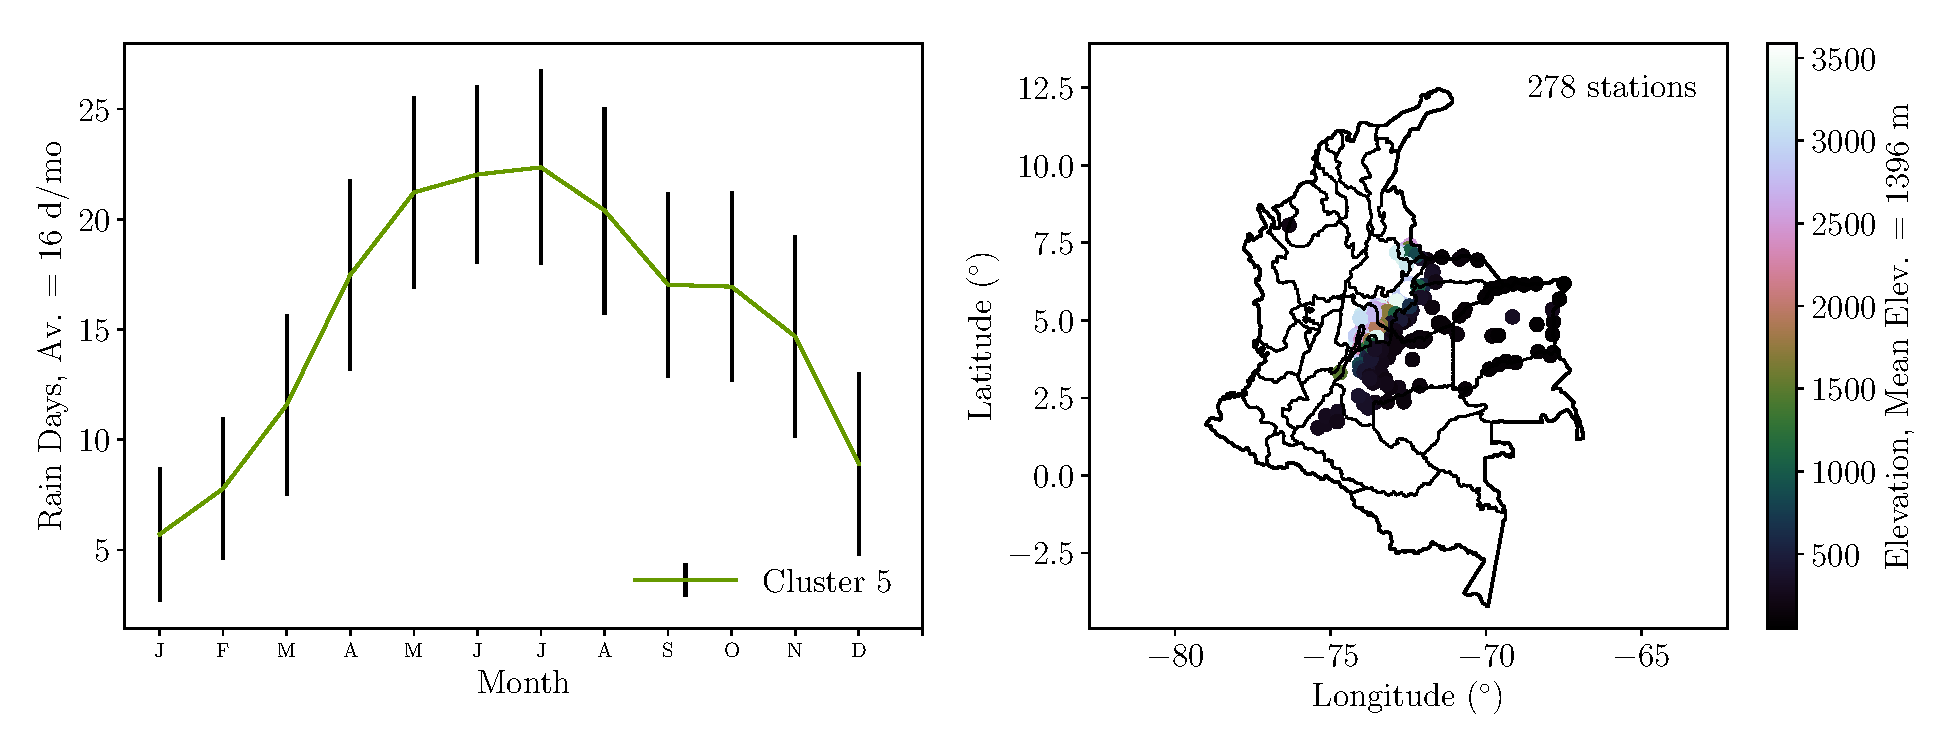
\includegraphics[scale=0.5]{gmmd4.pdf}
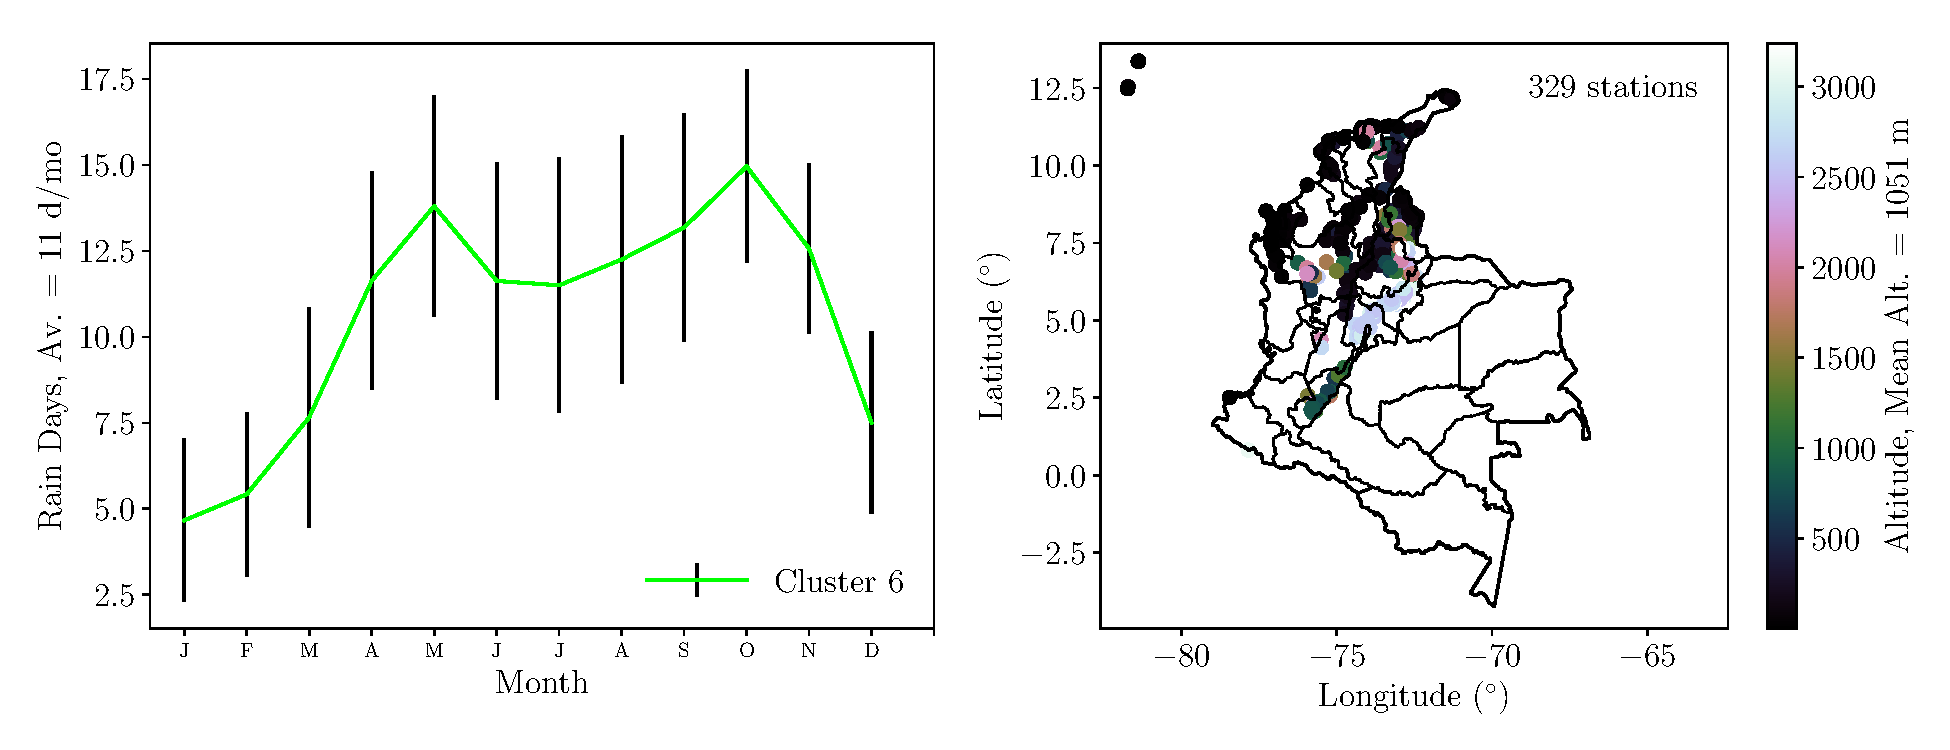
\includegraphics[scale=0.5]{gmmd5.pdf}
\caption{Climate clusters as predicted by the lowest-BIC Gaussian Mixture Model for rain days. Left column: Average monthly rain days and standard deviation (error bars) for each climate cluster. Right column: Geographical location and altitude of weather stations in each rain days cluster.}\label{clustl}
\end{center}
\end{figure}

\begin{figure}
\begin{center}
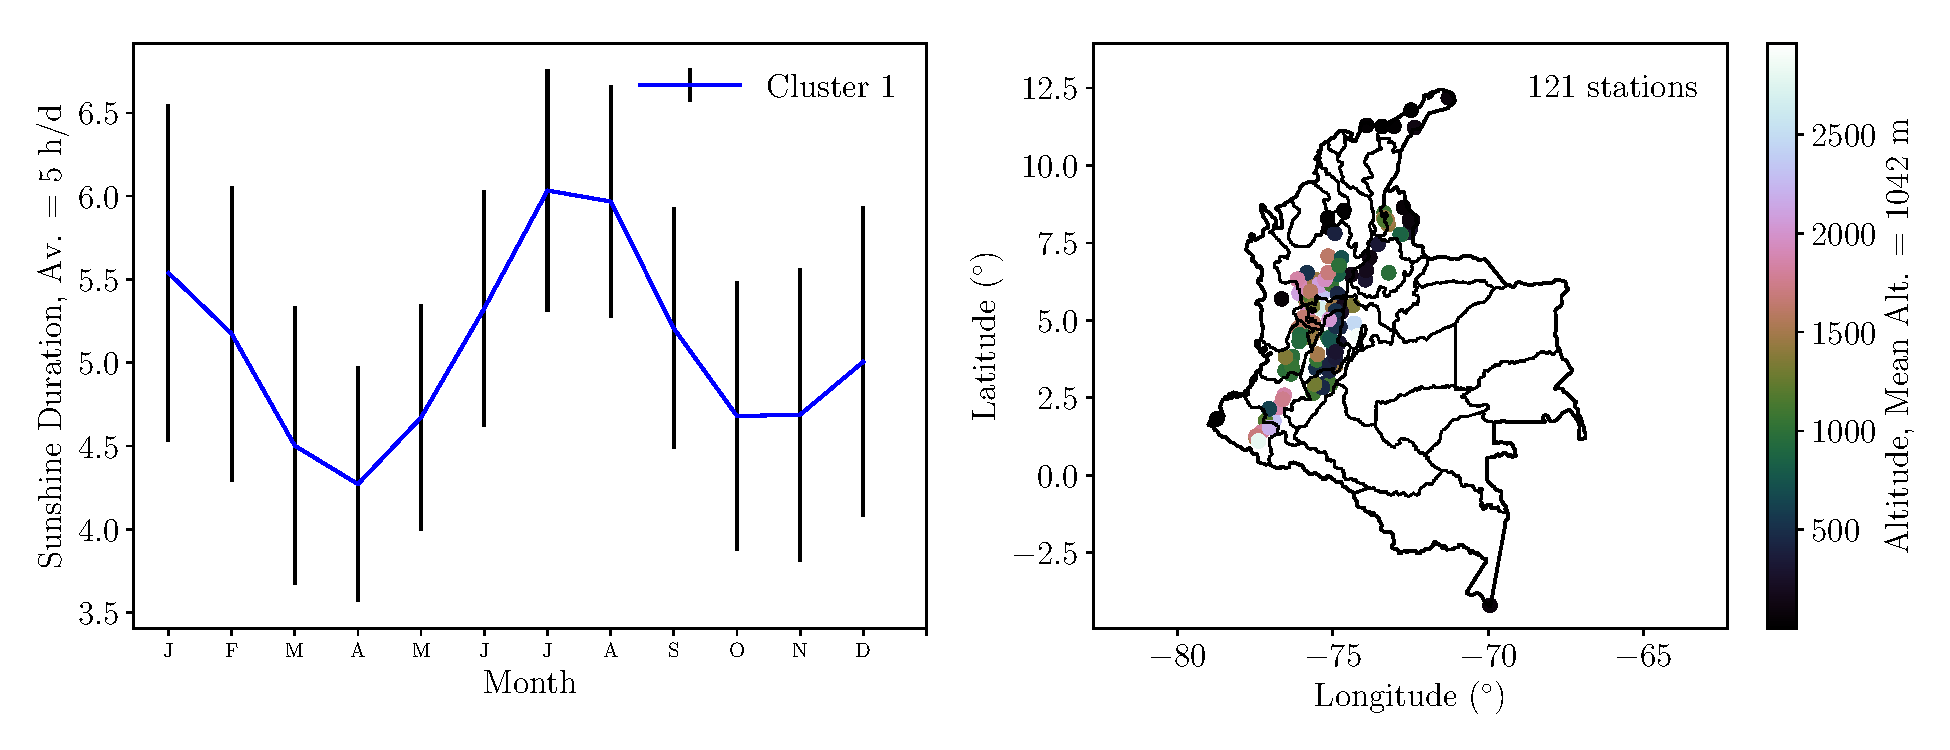
\includegraphics[scale=0.5]{gmmb0.pdf}
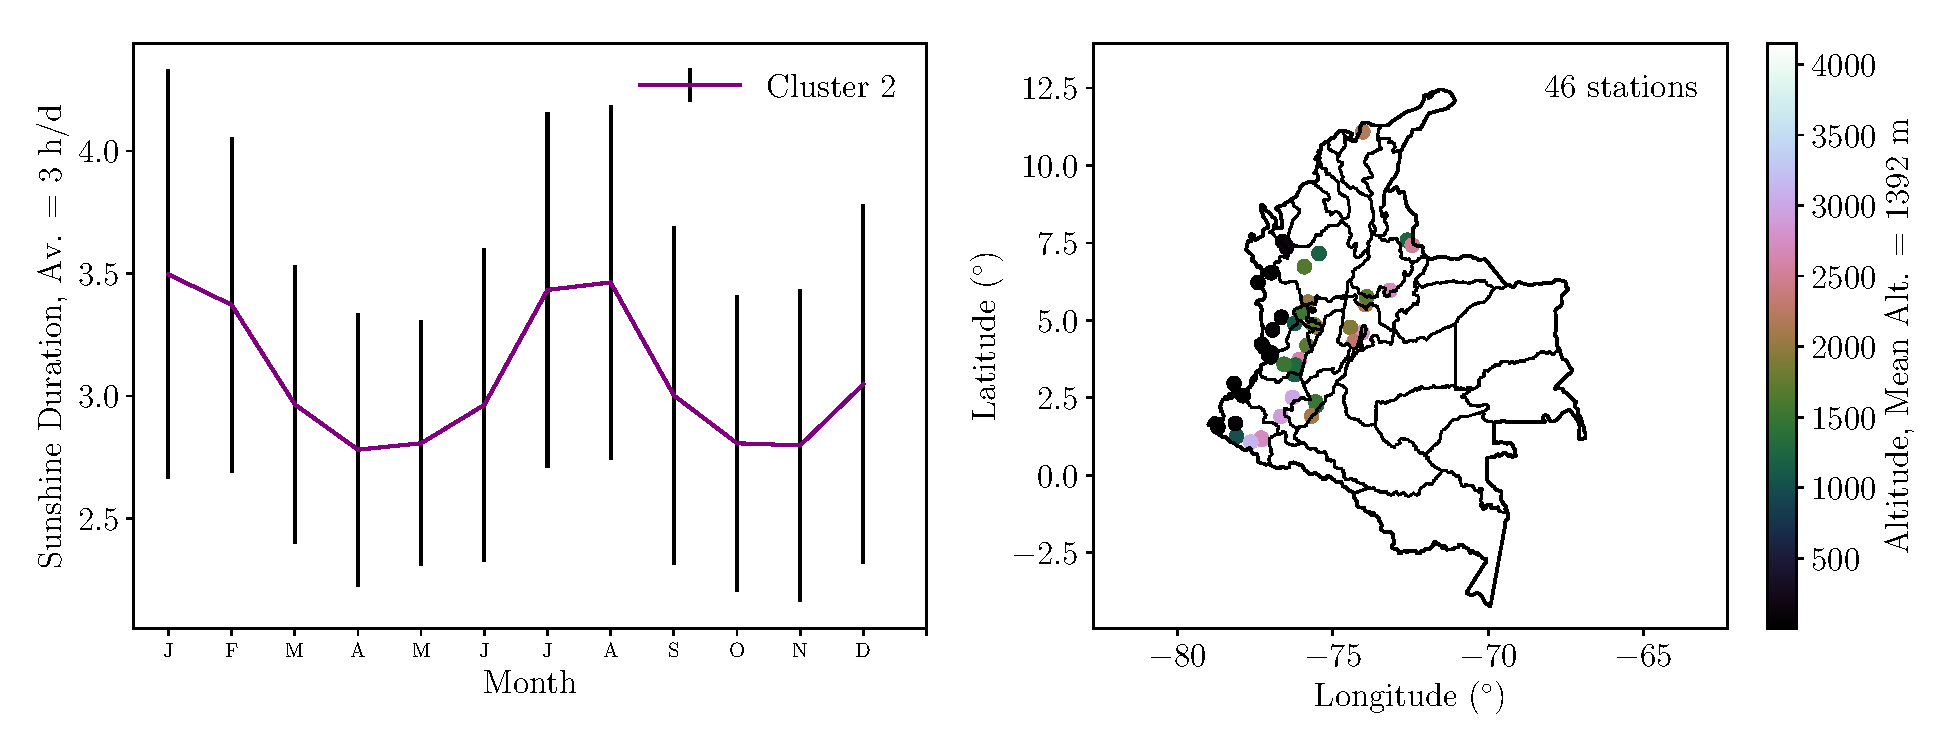
\includegraphics[scale=0.5]{gmmb1.pdf}
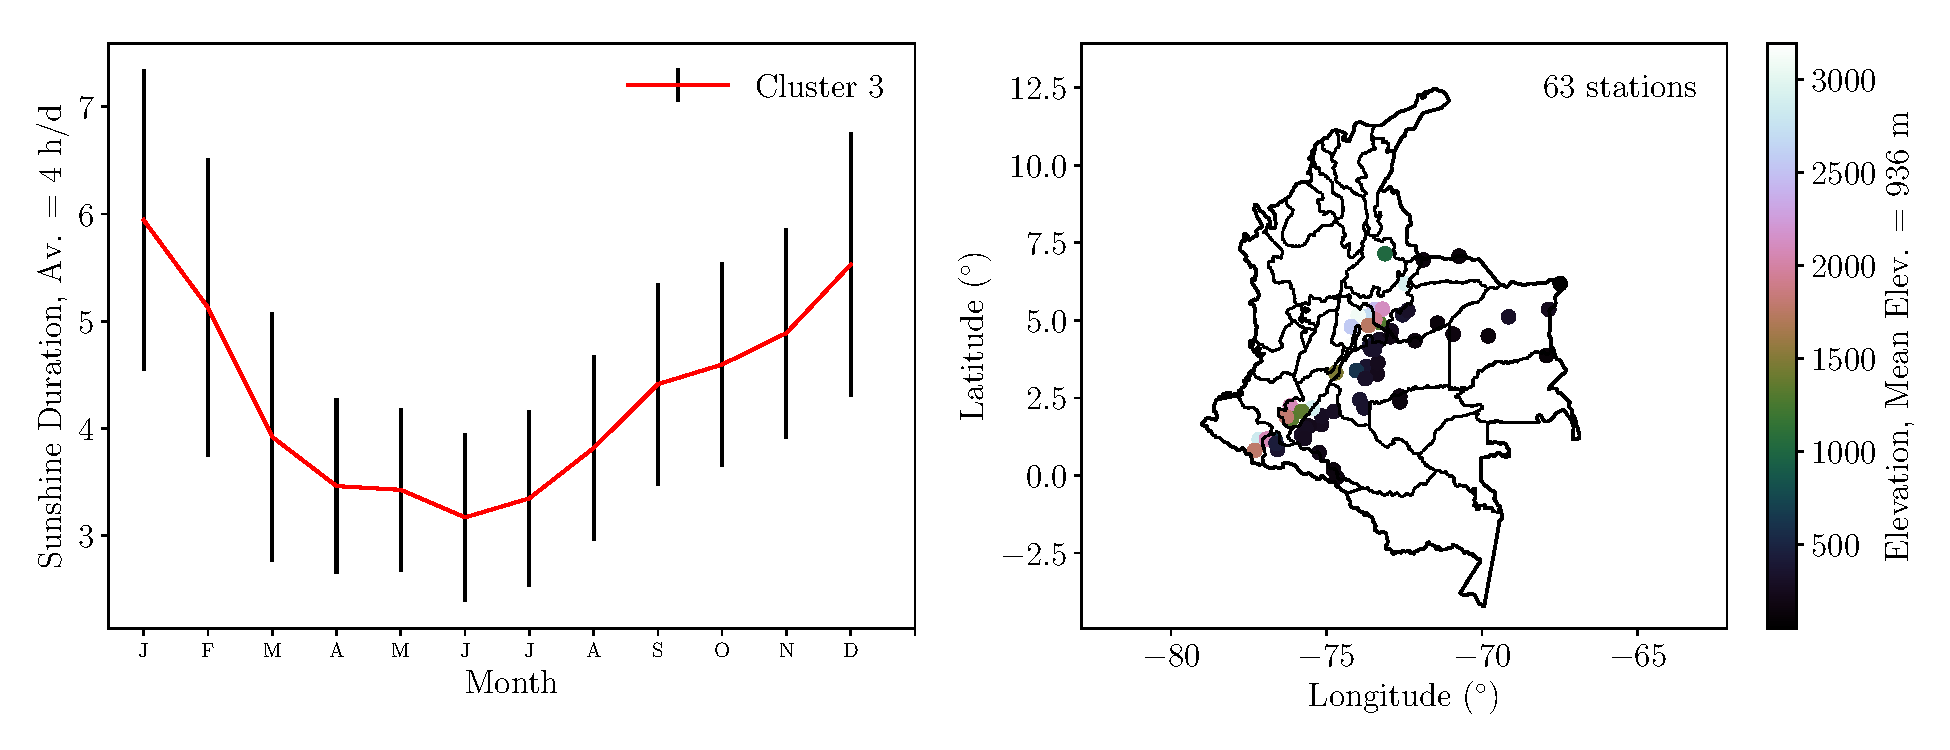
\includegraphics[scale=0.5]{gmmb2.pdf}
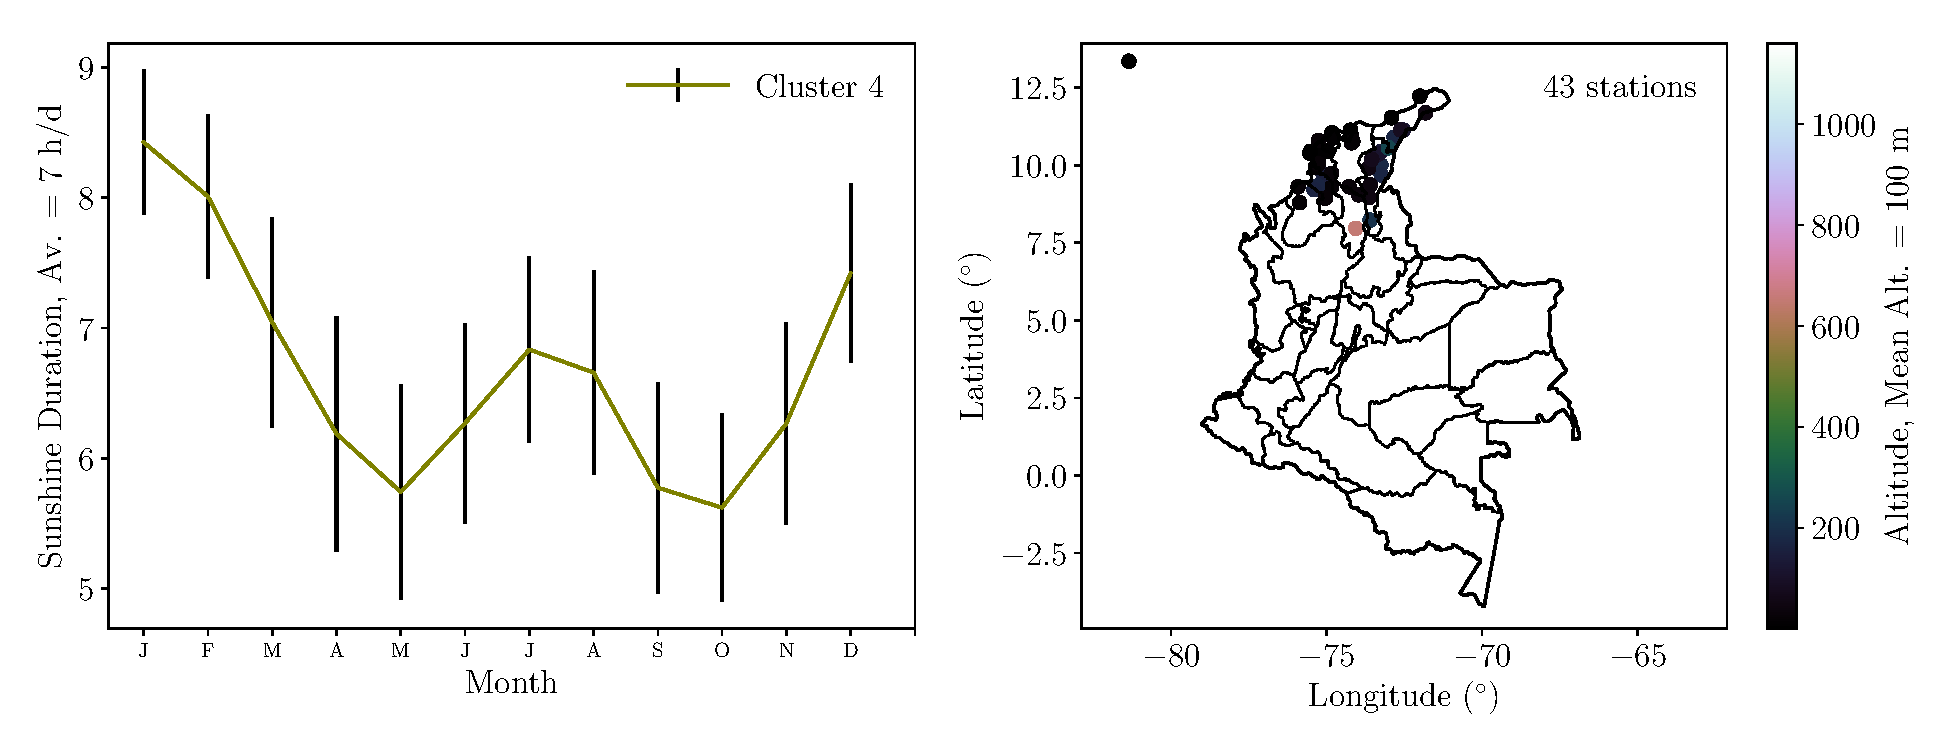
\includegraphics[scale=0.5]{gmmb3.pdf}
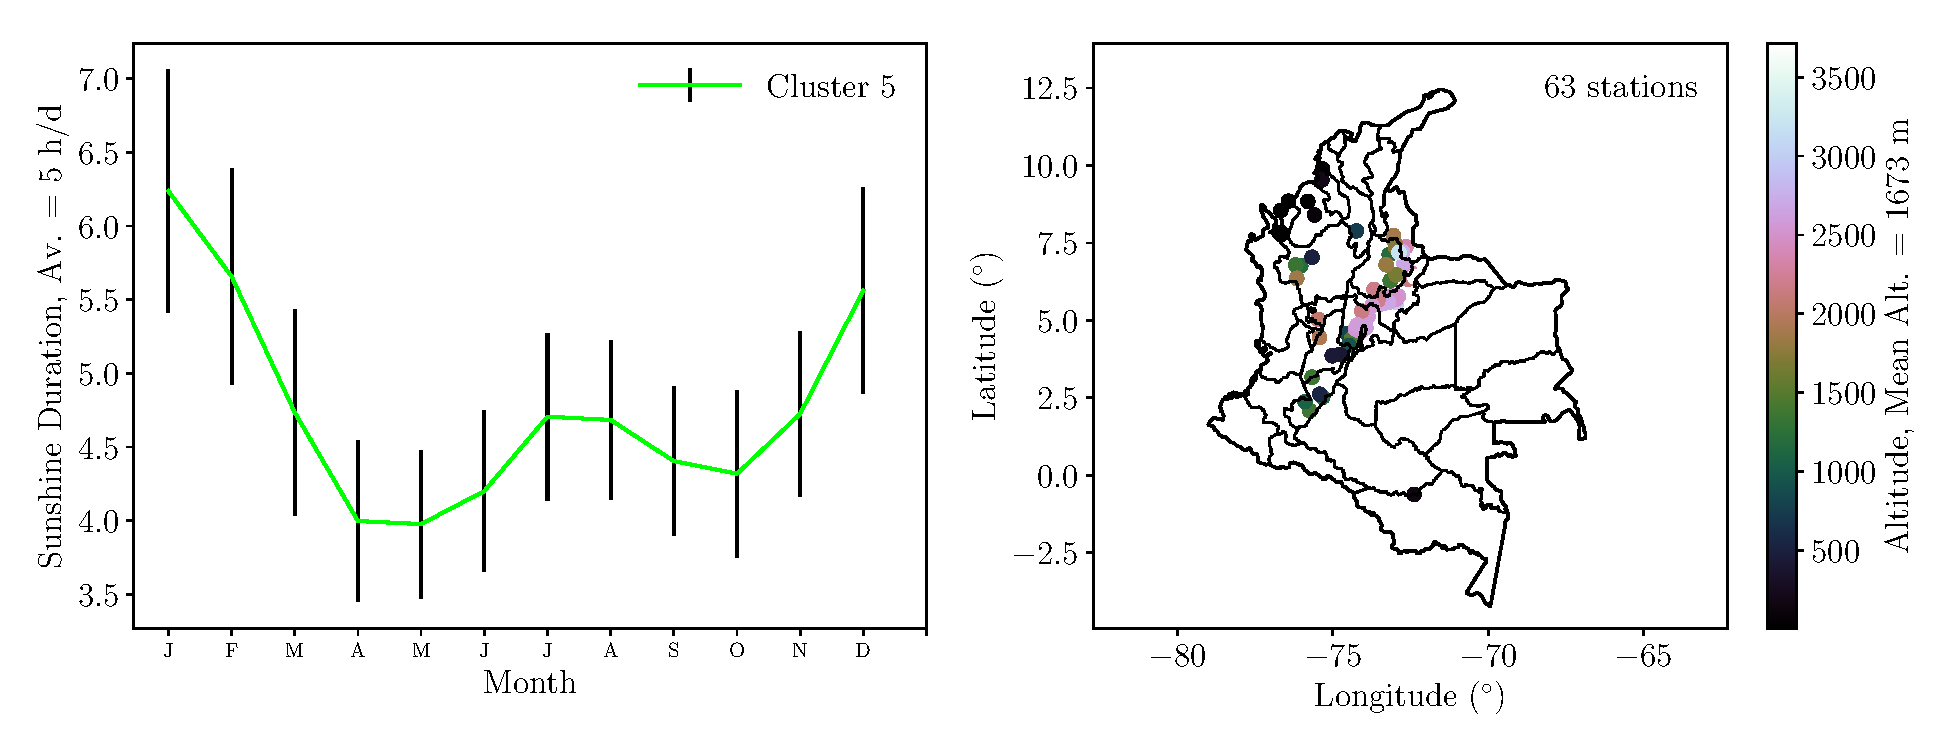
\includegraphics[scale=0.5]{gmmb4.pdf}
\caption{Climate clusters as predicted by the lowest-BIC Gaussian Mixture Model for sunshine duration. Left column: Average monthly sunshine duration and standard deviation (error bars) for each climate cluster. Right column: Geographical location and altitude of weather stations in each sunshine duration cluster.}\label{clustl}
\end{center}
\end{figure}

\begin{table}
\caption{\label{tabclu}Climate clusters according to a lowest BIC-based selection of Gaussian Mixture Models. See Figure \ref{bic}.}
\begin{indented}
\item[]\begin{tabular}{@{}lclll}
\br
Variable&Symbol&Lowest BIC&Lowest BIC&Preferred Clusters\\
&&No. of Clusters&Cov. Method &\\
\mr
Precipitation&$P$&11&Full&2,3,7,11\\
Rain Days&$D$&6&Full&1,4,6\\
Relative Humidity&$H$&2&Full&2\\
Sunshine Duration&$S$&5&Tied&1,4,5\\
\br
\end{tabular}
\end{indented}
\end{table}

\section{Discussion}

We wish to identify all stations for whom all four criteria (humidity, precipitation, rain days, sunshine duration) for identifying a region as having a stable sunny, dry climate can be met.  However, since only a few stations measured all variables, it is not straightforward to accept or reject stations based on their satisfing a criterion, i.e. belonging to one of our preferred clusters. This requires setting up a measure of quality for individual stations depending on their location and the variables they measured. We will describe the selection process and probabilistic analysis that allows us to quantify a station's capability for indicating regions with an unusually dry, sunny climate.\\

We start by creating a shortlist of stations that meet criteria for (and only for) the variables they measured. This means that if a station has precipitation and humidity data, it should belong to a humidity and precipitation cluster listed in Table \ref{tabclu} or else it is rejected. 665 stations across Colombia showed such behavior. However, since we are interested in high-mountain regions, we included a criterion for elevation limiting our list to 119 stations located above 2000 masl. This shortlist was further reduced by requiring that the total average plus 1$\sigma$ for precipitation, rain days, and relative humidity is less than 4.3 mm/d, 17 d/mo, and 81\% respectively, and for sunshine duration, more than 4 h/d for any given station. This left us with 83 weather stations. \\

However, we want to give a measure of the quality of the station vis-a-vis our criteria, i.e. a station that meets less than all four criteria should still be considered in our analysis, but it cannot be given the same importance as a station that meets all four criteria. In order to account for this, and controlling for the fact that stations are not distributed evenly in elevation (Figure \ref{totmap}b), we propose a quality measure based on a probabilistic analysis of the data.


\subsection{Probabilistic Analysis}

We base our analysis on the probability for our hypothesis that a station which appears in our shortlist meets all four criteria, given that it is located at a given elevation. We can write down this probability in terms of the following events:

\begin{itemize}
\item $C$ is the event that a given station meets all four criteria, i.e. belongs to our preferred clusters for the four variables relevant to this study.
\begin{itemize}
\item $C$ is actually the conjunction of all four of the $P,D,H,S$ events ``The station belongs to a preferred cluster for variable $X$'', i.e. $C=P\cap R\cap H \cap S$.
\end{itemize}
\item $A$ is the event that a given station appears in our shortlist.
\item $T_i$ is the event that a given station is of type $T_i$ (See Table \ref{tabstype}).
\begin{itemize}
\item For example, if $M_X$ is the event ``the station measured variable $X$'', then the event $T_7$ is equivalent to $M_P\cap \neg M_R\cap M_H \cap M_S$
\end{itemize}
\item $h$ is the event that a given station is located at an elevation $h$.
\end{itemize}

Thus, the probability that a station $j=(0,1,...,N_\mathrm{stations})$ of type $T_i$, meets all four criteria ($C$) and appears in our shortlist ($A$) given that it is located at an elevation $h$, can be written as $P_j=P(C\cap A\cap T_i\ |\ h)$. We cannot  calculate exactly this probability, as it depends on unknown unknowns, i.e. whether a station that did not measure a given variable in reality belongs to one of our preferred climatological clusters for that variable. Thus we will use Bayes' theorem to help estimate this probability using simpler conditional probabilities. First we control for the inhomogeneous distribution of elevations $P(h)$,
\begin{equation}
P(C\cap A\cap T_i\ |\ h)=\frac{P(C\cap A\cap T_i\cap h)}{P(h)}\ .
\end{equation}
The joint probability of all events $C\cap A\cap T_i\cap h$ can be rewritten as,
\begin{equation}
P(C\cap A\cap T_i\ |\ h)=\frac{P(h\ |\ C\cap A\cap T_i)}{P(h)}P(C\cap A\cap T_i)\ .
\end{equation}
If a station satisfies all four criteria, $P(C\cap A\cap T_i)=1$. This probability can be expressed in terms of simpler conditional probabilities,
\begin{equation}
P(C\cap A\cap T_i\ |\ h)=\frac{P(h\ |\ C\cap A\cap T_i)}{P(h)}P(C\ |\ A\cap T_i)P(A\ |\ T_i)P(T_i)\ .
\end{equation}
Here $P(h\ |\ C\cap A\cap T_i$ is the distribution of elevations for a station type ($T_i$) on our shortlist ($C\cap A$), $P(A\ |\ T_i)$ is the probability that a station of type $T_i$ is in our shortlist, $P(T_i)$ is the probability that a station type is $T_i$, and $P(C\ |\ A\cap T_i)$ is the probability that a station meets all four criteria ($C$) given that it is in our shortlist ($A$) and is of type $T_i$. All of these probabilities except for the last one can be computed directly from the data.  The probability $P(C\ |\ A\cap T_i)$ has to be estimated indirectly, as we cannot presume to know under which conditions a station can satisfy all our criteria. We can rewrite this probability as,
\begin{eqnarray}
P(C\ |\ A\cap T_i)&=P(P\cap D\cap H\cap S\ |\ A\cap T_i)\ , \\
\label{pclanti}
&=\frac{P(P\cap D\cap H\cap S\cap A\cap T_i)}{P(A\cap T_i)}\ . 
\end{eqnarray}
In order to estimate $P(C\ |\ A\cap T_i)$ we assume that the probability of a station meeting our criteria for a given number of variables is independent of the station type. To illustrate this, let us assume that a given station is of type 1, so it only measured precipitation and rain days, i.e.,
\begin{equation}
T_1=M_P\cap M_D\cap\neg M_H\cap\neg M_S\ .
\end{equation}
If this station of type $T_1$ is in our shortlist ($A$), the $P$ and $D$ criteria are met. Thus,
\begin{equation}
P(P\cap D\cap H\cap S\cap A\cap T_1)=P( H\cap S\ |\ A\cap T_1)\ .
\end{equation}
Substituting this into Eq. (\ref{pclanti}),
\begin{equation}
P(C\ |\ A\cap T_1)=\frac{P( H\cap S\ |\ A\cap T_1)}{P(A\cap T_1)}=P(H\cap S\ |\ A\cap T_1)
\end{equation}
The last term in the previous expression is unknown, but we can approximate it assuming, as mentioned above, that it is independent of the station type. Therefore, 
\begin{equation}
P(C\ |\ A\cap T_i)\simeq P(H\cap S)\ .
\end{equation}
The probability on the right hand side of the previous equation can be directly computed from the data, as it only requires counting how many stations meet both $H$ and $S$ criteria. This procedure can be extended to all other station types.\\

Since the probabilities for stations in our shortlist vary by orders of magnitude, for clarity's sake we decided to use a logarithmic quality index for a station in our shortlist. For $j=(0,1,...,N_\mathrm{stations})$,
\begin{equation}
Q_j=9\ \frac{\log (\nicefrac{P_\mathrm{j}}{P_\mathrm{min}})}{\log (\nicefrac{P_\mathrm{max}}{P_\mathrm{min}})}+1\ .
\end{equation}
Here $P_\mathrm{min},P_\mathrm{max}$ are the lowest and highest values for the probabilities for the stations in the first shorlist of 665 stations that satisfy criteria for all measured variables. Thus, if $P_j=P_\mathrm{max}$, $Q_j=10$, and if $P_j=P_\mathrm{min}$, $Q_j=1$.


\section{Results}

\begin{figure}
\begin{center}
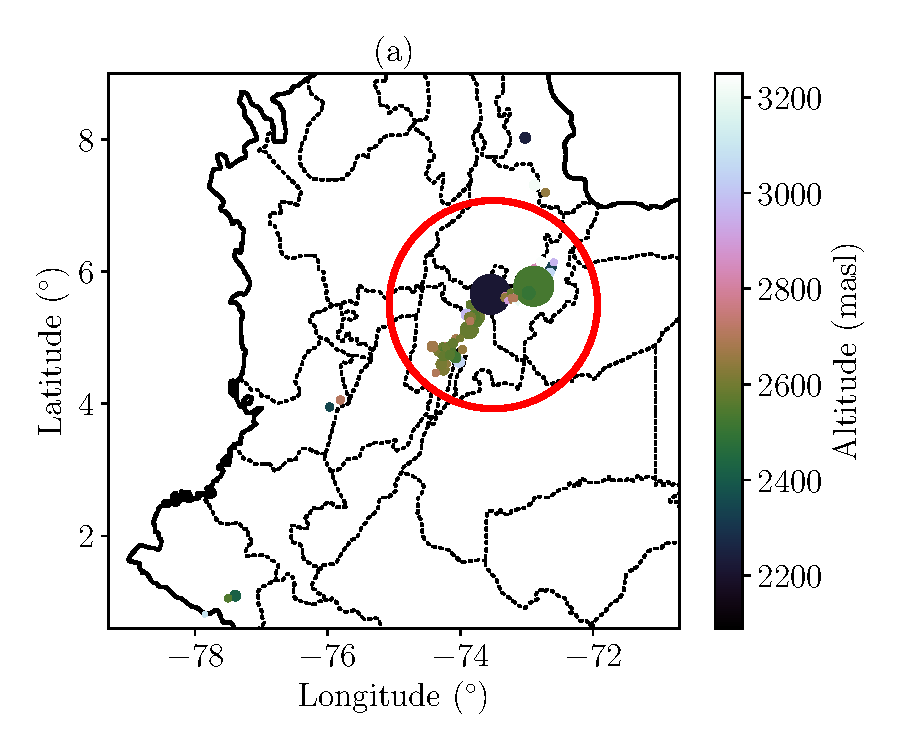
\includegraphics[scale=0.5]{slist.pdf}
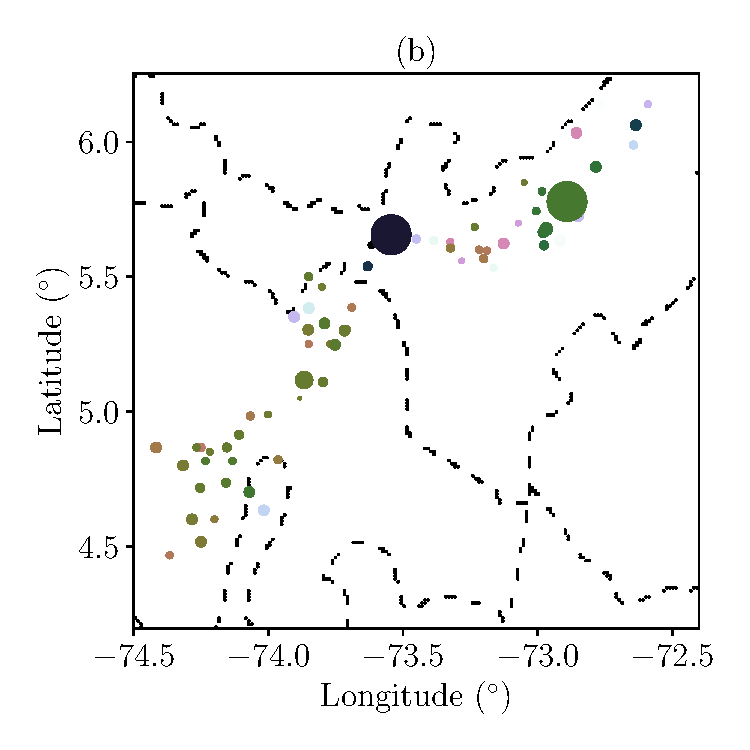
\includegraphics[scale=0.5]{slistz.pdf}
\caption{Map of stations in our final shortlist. The highlighted region on (a) is seen in more detail in (b), which corresponds approximately to the Colombian \emph{altiplano} region. Marker size is proportional to the probability $P_j$, where the largest points correspond to a $Q_j=10$.}\label{shortlist}
\end{center}
\end{figure}

We selected clusters of climatologically similar stations across Colombia using an unsupervised learning low-dimensional embedding algorithm for each measured variable. From these clusters, 83 weather stations came up as potential candidates for identifying high-mountain sites (at an elevation greater that 2000 masl) with an unusually dry, sunny weather.\\

Given that many of our candidate stations were lacking in relative humidity and sunshine duration data, we extrapolated using data from nearby stations (at less than 4 km away and at an elevation difference of less than 100 m). We made sure that in general, for stations less than 5 km away, the difference in relative humidity and sunshine duration data are less than 15\%. The extrapolated data suggested that 4 of the stations in the shortlist did not satisfy the relative humidity and sunshine duration criteria.  The remaining 79 stations are mapped in Figure \ref{shortlist}a.\\

All stations outside of the region located within the latitude, longitude range $[(4.3,6.2),(-72.4,-74.5)]$ seem to be outliers, and while they could indicate unusually dry, sunny regions, there are not enough stations nearby to say anything conclusively as can be seen in Figure \ref{outliers}. Furthermore, those stations only measured precipitation ($Q_j=2.2$), which leads us to reject them from our shortlist. \\
%The points of interest outside this region are too sparsely located to suggest a candidate region of interest, \\

The final 70 stations located nearby the Cundinamarca-Boyac\'a region of Colombia are shown in more detail in Figure \ref{shortlist}b. This figure shows two candidate locations in the northern region (Boyac\'a department), where the quality index $Q_j$ (proportional to the point size) indicates that all four criteria are satisfied. In order to see if those regions are geographically correlated, we grouped together these stations in a simplified manner using a lowest-BIC spherical covariance Gaussian Mixture Model on their coordinates \ref{geobic}.\\



\begin{figure}
\begin{center}
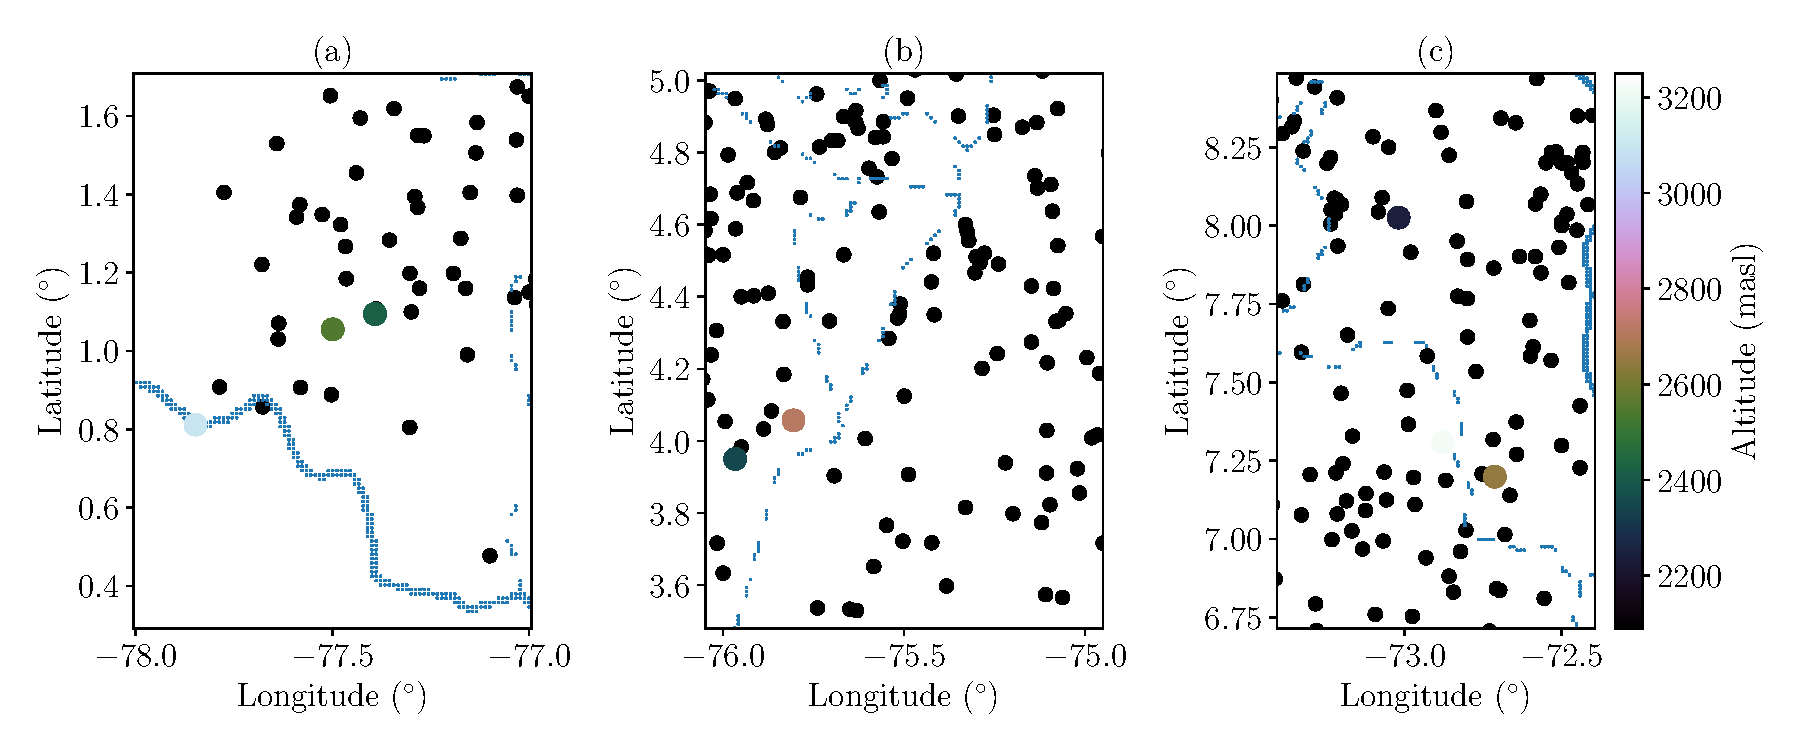
\includegraphics[scale=0.55]{outliers.pdf}
\caption{Map of stations in our final shortlist but outside of the Colombian \emph{altiplano} region highlighted in Figure \ref{shortlist}. Marker size is proportional to the Probability $P_j$, where the smallest points correspond to a $Q_j=2.2$.}\label{outliers}
\end{center}
\end{figure}

\begin{figure}
\begin{center}
\includegraphics[scale=0.55]{geobic.pdf}
\includegraphics[scale=0.55]{geobic2.pdf}
\caption{Results  for a lowest-BIC spherical covariance Gaussian Mixture Model geographical clustering on the stations located inside the red circle in Figure \ref{shortlist}b. (a) BIC results for different number of clusters. (b) Lowest-BIC GMM geographical clustering classification.}\label{geobic}
\end{center}
\end{figure}

 show 6 candidate regions we plotted the predicted variance regions for each cluster along with other stations in our sample (rejects) in Figure \ref{latlonreg}. From this figure, we can reject regions where the number of rejected stations within the predicted variance regions is similar to or higher than the number of stations in our shortlist for a specified cluster.

\subsection{La Sabana}

The region located to the west of Bogot\'a is a hilly region at an elevation above 2600 masl, with a large variety of microclimates, which explains the significant amount of stations from this region in our shortlist. However, Figure \ref{lasabana} shows that within this predicted variance region there are more stations that do not satisfy our criteria than stations that do. Furthermore, stations that meet and do not meet our criteria are homogeneously distributed. This, compounded with the fact that most (70\%) of these stations have a $Q$ value lower than 5.6 due to the lack of humidity/sunshine data, implies that at the moment this is not a strong candidate region of interest.
%light blue
\subsection{Valle de Ubat\'e}

This region, located to the NNE of Bogot\'a s a hilly region along a valley at an elevation above 2600 masl. The ratio of number of stations that do not meet our criteria to the stations in this predicted variance region is low (0.3), and almost half of these stations (\%46) have a $Q$ value higher than 6. This indicates a potential candidate region, although more  sunshine and humidity data are needed. In our next paper we will study the amount of atmospheric water vapor near this region.
%cyan

\subsection{Villa de Leyva}

The region near the town of Villa de Leyva is known for its dry weather, and the stations located within this region seem to support this belief. The ratio of stations not in our shortlist vs. the stations in this predicted variance region is not very low (0.4). However, Figure \ref{villadeley} seems to indicate that the actual region of interest is narrower than the predicted variance region, as the stations that do not satisfy our criteria are on the NNW and SSW fringes of said region. The presence of one very high-$Q$ station is very suggestive of this region being a strong candidate. However, its relatively low elevation (near 2200 masl) can signify the presence of too much atmospheric water vapor above the surface. This will be covered in our next paper.
%red

\subsection{Tunja Canton}

The variance predicted region west of Tunja is located in the historic Tunja Canton, and even though the ratio of stations not in our shortlist to stations in this predicted region is low (0.31), there are simply not enough humidity and sunshine data to make any strong conclusion regarding this region. However, the high-elevation location of some of these stations is tantalizing, which is why we will keep this as a region of interest for our next paper.

% dark blue

\subsection{Valle del Sol}

This is one of the most promising regions in our sample. Located in a wide, sunny valley (hence the name) at an elevation of 2600 masl, it is surrounded by mountains, and rains are not as common as elsewhere in the country. This region has the lowest ratio of not in our shortlist stations to stations in this predicted variance region (0.2), $\%40$ of the stations have a $Q$ value higher than 6, and one of the stations has a very high-$Q$ value. This will be one of the regions of interest for our next paper, and we think that it warrants radiometer measurements to be carried out.

\subsection{Pisba National Park}

This is a \emph{p\'aramo} region, characterized by high-mountain tundra weather. The ratio of stations not in our shortlist to station in this predicted variance region is high (0.5), and it is unlikely that the mist allows for a low-atmospheric water vapor region to be located here, even if rain is sporadic. The lack of a high-$Q$ station means that more sunshine-humidity data are needed, but this is possibly not a region of interest.\\

%figures for all these

% tables for our three favorites, Ubat\'e, Villa, Sol.

One, to the NWW of Bogot\'a, another to the N of Bogot\'a, in the region known as Valle de Ubat\'e, \\

4000 masl might be interesting as well, but there are not enough stations.\\

Seasonality plots\\

 


  

 \section*{References}
 \bibliography{paperclimate}
\bibliographystyle{jphysicsB}
  
  \end{document}